%!TEX root = ./presentation.tex
%&presentation.fmt

%!TEX root = ./presentation.tex 
\scrollmode

\documentclass[aspectratio=169]{beamer}
\usetheme{Madrid}


% -------------- COMPILE VARIABLES --------------
\newif\ifINTRO

\INTROfalse      % Build only intro slide


% ------------------ VARIABLES ------------------
\newcommand{\userName}{Pascal-Emmanuel Lachance \&\\Maxime Grenier-Castillo}
\newcommand{\initials}{P-E.L \& M. G-C}
\newcommand{\projectName}{Comment se Propage un Signal Électro-Magnétique?}


% Le Parfait Petit Manuel Pluridisciplinaire et Multidisciplinaire
% Pour les PCB Multicouches Prototypables et Manufacturables
% Par Petit Maxime et Petit Pascal
% Par le Moyen d'une Présentation Procédurale PowerPoint Multimédia sur les PCB en Présentiel
% Pour les Misérables Pragmatiques

\newcommand{\institution}{C3i}
\newcommand{\repo}{PPPPP}
\newcommand{\user}{raesangur}
\newcommand{\docName}{Presentation}

\author{\userName}
\title{\projectName}
\subtitle{PPMPMPPMPMPPMPPPMPPPMPPPMP05}
\institute{Compétitions de Conception de Circuits Imprimés}
\date{\today}


% ----------- CONFIGURATION INCLUDES ------------
%!TEX root = ../presentation.tex

%%%%%%%%%%%%
% PACKAGES %
%%%%%%%%%%%%

% =============== General Formatting ============
\usepackage[T1]{fontenc}
\usepackage{lmodern}
\usepackage{pifont}
\usepackage{amsmath}
\usepackage{amssymb}
\usepackage{fontawesome5}
\usepackage{comment}
\usepackage{adjustbox}
\usepackage{array}
\usepackage{multicol}
\usepackage[yyyymmdd]{datetime}

% =============== Colors ============
\usepackage{colortbl}
\usepackage[many]{tcolorbox}
\usepackage{xcolor}
\usepackage{hyperref}

% =============== Math ============
\usepackage{mathtools}
\usepackage{nicefrac}
\usepackage{siunitx}
\usepackage{calc}

% =============== Figures ============
\usepackage{tikz}
\usepackage{circuitikz}
\usepackage{pgfplots}
\usepackage{animate}
\usepackage{environ}

% =============== Listings ============
\tcbuselibrary{listings}      % Raesangur
\usepackage{listings}         % Main package for inserting code
\tcbset{listing engine={listings}}
\usepackage[scaled]{beramono} % For using the beramono font


% =============== Bibliography ============
%\usepackage{cite}

\usepackage[style=alphabetic,backend=biber, style=numeric, sorting=none]{biblatex}
%\addbibresource{references.bib}
\renewcommand*{\mkbibacro}[1]{#1}




% =============== Package Setup ============
\newcolumntype{C}[1]{>{\centering\arraybackslash}p{#1}}

\renewcommand{\dateseparator}{--}

\newcommand{\cmark}{\ding{51}} % ✓
\newcommand{\xmark}{\ding{55}} % ✗


% ------ Tikz ------
\usetikzlibrary{arrows, shapes, calc, positioning}
%\usetikzlibrary{external}
%\usepgfplotslibrary{external}
%\tikzexternalize
\pgfplotsset{compat=1.18}
%!TEX root = ../presentation.tex


% -------------- BACKGROUNDS --------------

\newcommand\titlebackground {
    \usebackgroundtemplate{
    \begin{tikzpicture}[remember picture, overlay]
        \node[at=(current page.center)] {
            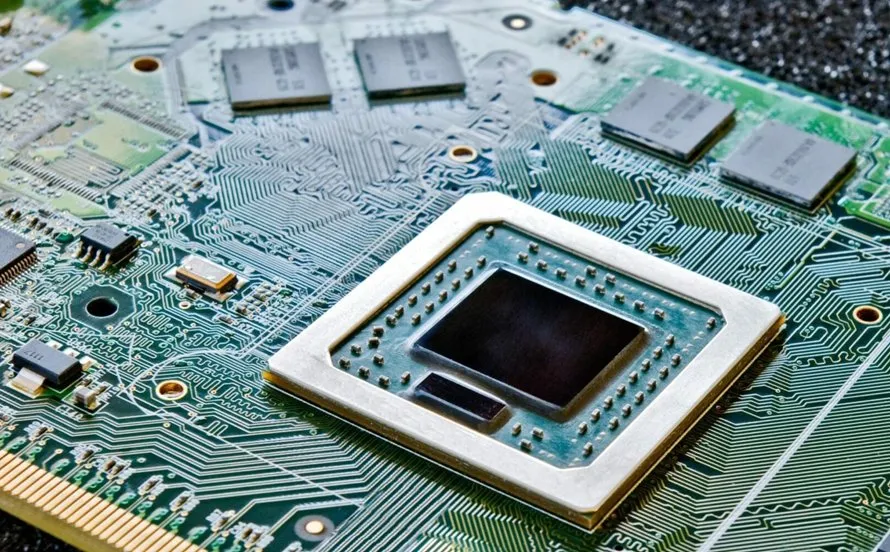
\includegraphics
            [width=\paperwidth, keepaspectratio]
            {pictures/background/background-PCB.png}
        };
    \end{tikzpicture}
    }
}


\newcommand\introbackground {
    \usebackgroundtemplate{
    \begin{tikzpicture}[remember picture, overlay]
        \node[at=(current page.center)] {
            
\includegraphics
            [width=\paperwidth, keepaspectratio]
            {pictures/background/background-pcb-poster.png}
        };
    \end{tikzpicture}
    }
}

\newcommand\defaultbackground {
    \usebackgroundtemplate{
    \begin{tikzpicture}[remember picture, overlay]
        \node[at=(current page.center)] {
            
\includegraphics
            [width=\paperwidth, keepaspectratio]
            {pictures/background/background5.pdf}
        };
    \end{tikzpicture}
    }
}


% -------------- TITLE PAGE --------------
\makeatletter
\setbeamertemplate{title page}
{
    \begin{columns}
        \begin{column}{0.75\textwidth}
            {
                
\includegraphics[scale = 0.35]{pictures/logo/udes_logo.pdf}\\
            }
            \vspace{24pt}
            \begin{tikzpicture}
                \def\boxwidth{\textwidth}
                \def\boxheight{3cm}
                \def\cornerradius{6pt}
                \def\shadowshift{0.5ex}
                
                \node[fill=UDSgreenSolidarite,
                      fill opacity=0.9,
                      rounded corners=6pt,
                      minimum width=\boxwidth, minimum height=\boxheight,
                      text=white,
                      text opacity=1,
                      align=center] (mainbox) at (0, 0){
                    \usebeamerfont{title}
                    \textbf{\inserttitle}\\
                    \usebeamerfont{subtitle}\usebeamercolor[fg]{subtitle}
                    \textbf{\insertsubtitle}\\\\
                    \small\usebeamerfont{author}\insertauthor
                };

                \path (mainbox) node[rectangle, minimum width=0.999\boxwidth, minimum height=0.996*\boxheight, rounded corners=\cornerradius, save path=\inbox] at (0, 0) {};
                \tikzset{protect=\inbox}

                \begin{scope}[transparency group, opacity=1]
                    \fill[color=black, opacity=0.33, rounded corners=\cornerradius,
                          blur shadow = {shadow xshift=.25ex, shadow yshift=-.25ex}]
                        (-0.5\boxwidth + \shadowshift, 0.5*\boxheight - \shadowshift) rectangle 
                        (0.5\boxwidth + \shadowshift, -0.5*\boxheight - \shadowshift);
                \end{scope}
            \end{tikzpicture}
            \vspace{24pt}
        \end{column}
        \begin{column}{0.25\textwidth}
        \end{column}
    \end{columns}
}
\makeatother


\newcommand\thankyouframe{
    \begin{frame}
    \begin{multicols}{2}
        \begin{beamercolorbox}[sep=8pt, center, shadow=true, rounded=true, wd=0.5\textwidth, bgopacity=0.85]{title}
            \usebeamerfont{title}Merci!\\
        \end{beamercolorbox}%
    \vfill\null
    \columnbreak
    \end{multicols}
\end{frame}
}

%!TEX root = ../presentation.tex



% Insert a figure with optional scaling and caption.
% 1: Width as a fraction of \textwidth   (default: 1)
% 2: Height as a fraction of \textheight (default: 0.8)
% 3: Caption text (optional)
% 4: Filename of the image (relative to 'pictures/' directory, no extension needed)
%
% Example:
% \makefigure[0.9][0.5][A sample image]{example-image}
\NewDocumentCommand{\makefigure}{O{1} O{0.8} o m}{%
    \begin{figure}%
        \centering%
        \includegraphics%
            [width=#1\textwidth, height=#2\textheight, keepaspectratio, page=1]%
            {pictures/#4}%
        \IfValueTF{#3}{%
            \caption*{#3}%
        }{}%
    \end{figure}%
}


% Insert a figure with border and with optional scaling and caption.
% 1: Width as a fraction of \textwidth   (default: 1)
% 2: Height as a fraction of \textheight (default: 0.8)
% 3: Caption text (optional)
% 4: Filename of the image (relative to 'pictures/' directory, no extension needed)
%
% Example:
% \makefigureborder[0.75][0.7][A sample image]{example-image}
\NewDocumentCommand{\makefigureborder}{O{1} O{0.8} o m}{%
    \begin{figure}%
        \centering%
        \tcbox[colframe=accent, colback=background]{
            \includegraphics%
                [width=#1\textwidth, height=#2\textheight, keepaspectratio, page=1]%
                {pictures/#4}%
            \IfValueTF{#3}{%
                \caption*{#3}%
            }{}%
        }
    \end{figure}%
}


% Create a TikZ circuit figure with adjustable size.
% 1: Width as a fraction of \textwidth   (default: 1)
% 2: Height as a fraction of \textheight (default: 0.8)
%
% Example:
% \begin{maketikzfigure}[0.7][0.5]
%     \draw (0,0) to[battery] (0,2);
% \end{maketikzfigure}
\NewDocumentEnvironment{maketikzfigure}{O{1} O{0.8}}{%
    \vspace{-16pt}%
    \begin{center}%
        \begin{adjustbox}{width=#1\textwidth, height=#2\textheight, keepaspectratio}%
            \begin{circuitikz}[american voltages]%
}
{%
            \end{circuitikz}%
        \end{adjustbox}%
    \end{center}%
}




% Begin a two-column layout with adjustable left column width.
% 1: Width of the left column as a fraction of \textwidth (default: 0.5)
%    The right column will take the remaining space after the left column
%
% Example:
% \begin{twocolumns}[0.6]
%   \leftcol
%     Left side content.
%   \rightcol
%     Right side content.
% \end{twocolumns}
\NewDocumentEnvironment{twocolumns}{O{0.5}}{%  
  \def\leftcolwidth{#1\textwidth}%
  \def\rightcolwidth{\dimexpr \textwidth - #1\textwidth\relax}%
  
  \begin{columns}%
}{%
  \end{column}%
  \end{columns}%
}

\NewDocumentCommand{\leftcol}{}{%
  \begin{column}{\leftcolwidth}%
}

\NewDocumentCommand{\rightcol}{}{%
  \end{column}%
  \begin{column}{\rightcolwidth}%
}


% Color an icon
% 1: Color name   (optional, default: accent)
% 2: Icon command (e.g., \faCheck)
%
% Example:
% \icon{\faCheck}
% \icon[red]{\faTimes}
\newcommand{\icon}    [2][accent] {\textcolor{#1}{#2}}

% Display an icon at the start of a list item with customizable color and spacing.
% 1: Color name       (optional, default: accent)
% 2: Horizontal space (optional, default: -12pt)
% 3: Icon command     (e.g., \faCheck)
%
% Example:
% \item[] \itemicon           {\faCheck}
% \item[] \itemicon[gray]     {\faCircle}
% \item[] \itemicon[red][-6pt]{\faTimes}
\NewDocumentCommand{\itemicon}{O{accent} O{-12pt} m}{\hspace{#2}\icon[#1]{#3}}



% Create a two-column list using a tabular environment.
% 1: Font size or formatting command (optional, default: \normalsize)
% 2: Row spacing via \arraystretch   (optional, default: 1.25)
% 3: Tabular column format           (optional, default: c l)
%
% Example:
% \begin{makelist}[\small][1.5]
%   \item{\faCheck} & Item one \\
%   \item{\faTimes} & Item two \\
% \end{makelist}
\NewDocumentEnvironment{makelist}{O{\normalsize} O{1.25} O{c l}}{%
    #1%
    \renewcommand{\arraystretch}{#2}%
    \begin{tabular}{#3}%
}{%
    \end{tabular}%
    \renewcommand{\arraystretch}{1}%
}

%!TEX root = ../presentation.tex

% =============== Colors ============
\definecolor{UDSgreenDurable}{RGB}{149, 193, 78}
\definecolor{UDSgreenVivacite}{RGB}{121, 181, 81}
\definecolor{UDSgreenCreativite}{RGB}{90, 173, 85}
\definecolor{UDSgreenFierte}{RGB}{0, 167, 89}
\definecolor{UDSgreenSolidarite}{RGB}{61, 143, 88}
\definecolor{UDSgreenBienEtre}{RGB}{68, 124, 90}
\definecolor{UDSgreenReussite}{RGB}{72, 106, 92} 
\definecolor{UDSgrey}{RGB}{228, 232, 225} 

\setbeamercolor{palette primary}{bg=UDSgreenSolidarite,fg=white}
\setbeamercolor{palette secondary}{bg=UDSgreenFierte,fg=white}
\setbeamercolor{palette tertiary}{bg=UDSgreenCreativite,fg=white}
\setbeamercolor{palette quaternary}{bg=UDSgreenReussite,fg=white}
\setbeamercolor{structure}{fg=UDSgreenReussite} % itemize, enumerate, etc
\setbeamercolor{section in toc}{fg=UDSgreenBienEtre} % TOC sections
\setbeamercolor{background canvas}{bg=UDSgrey}


\colorlet{foreground}{black}
\colorlet{background}{UDSgrey}
\colorlet{header}{UDSgreenSolidarite}
\colorlet{accent}{UDSgreenFierte}
\colorlet{accent2}{red}



% =============== Math ===============
\sisetup{
  per-mode=fraction,
  fraction-function=\nicefrac,
  detect-weight=true,
  detect-family=true
}

\DeclareSIUnit\bit{b}
\DeclareSIUnit\bits{bits}
\DeclareSIUnit\dbm{dBm}
\DeclareSIUnit\baud{baud}
\DeclareSIUnit\mil{mil}
\DeclareSIUnit\inch{in}

%!TEX root = ../presentation.tex


% ----------------- INLINE CODE -----------------

% Display monospace text in a grey box. Similar to ` text in markdown.
% 1: Color of the text in the textbox - default: [black]
% 2: Text to display
% 3: Following punctuation
%
% Note: This command sometimes continues in the margins of the page, 
% putting the punctuation as the 3rd argument prevents the following punctuation
% to be alone at the start of the next line.
%
% Example:
% This is an \inline{example}{,} without a specified color.
% This is another \href{https://www.example.com}{\inline[blue]{example}{.}}
\newcommand{\inline}[3][black]{ %
  \hspace{-8pt}%
  \begingroup%
  \raggedright%
  {
    \mbox{%
      \raggedright\tcbox[on line,%
                         boxsep=4pt, left=-1pt,right=-1pt,top=-4pt,bottom=-4.5pt,%
                         opacityframe=0, colback=gray!50,%
                         fontupper={\strut},%
                         enhanced, breakable]%
      {%
        \raggedright\lstinline[basicstyle=\ttfamily\small\color{#1},%
                               breaklines=true, breakatwhitespace=true,%
                               moredelim={[s][\ttfamily]{_}{_}}]%
      {#2}%
      }#3%
    }%
  }
  \endgroup%
  \hspace*{-8pt}~%
}


% --------------- REGULAR LISTING ---------------

% Create a lstlisting environment with custom syntax highlighting.
% 1: Syntax highlighting language - default: [logbook]
% 
% Note: The syntax highlighting argument is currently unused, as no other styles than logbook have been defined.
%
% Example:
% \begin{makelisting}{python}
% if __name__ == "__main__":
%     print("Example")
% \end{makelisting}
\lstnewenvironment{makelisting}[2][]
{
  \vspace{-8pt}
  \lstset{style=logbook #1}
}
{
  \vspace{-12pt}
}

% Create two aligned columns with proper spacing.
% Used to compare two listings or figures easily.
%
% Example:
% \begin{makecompare}
%   This is the first example, on the left.
%   \newcol
%   This second example is on the right!
% \end{makecompare}
\newenvironment{makecompare}
{
  \vspace{-1.25\cringlineskip}
  \begin{multicols}{2}
}
{
  \end{multicols}
  \vspace{-2\cringlineskip}
}


 % ----------------- CODE BLOCK -----------------
% https://tex.stackexchange.com/a/468526
\newtcbinputlisting[auto counter, list inside = lol, list type = {lstlisting}]{\makecode}[3][logbook]{
  breakable,
  listing file = {code/#3},
  listing options={style = logbook},
  listing only,
  boxrule = 1pt,
  title = {\textbf{Code \thetcbcounter:} \textbf{#2} \hfill \textbf{#3}},
  label = code:#3
}


% ---------------- CODE FORMATS -----------------
\lstdefinestyle{logbook}{
  escapeinside={<@}{@>},
  language=C,
  aboveskip=0.5cm,
  breakatwhitespace=false,
  breaklines=true,
  numbers=left,
  numbersep=8pt,
  numberfirstline = false,
  linewidth=\textwidth,
  stepnumber=1,
  frame=lines,
  framesep=0pt,
  framerule=0pt,
  framextopmargin=3pt,
  framexbottommargin=3pt,
  framexleftmargin=0.4cm,
  xleftmargin={0.75cm},
  rulecolor=\color{Black},
  rulesep=.4pt,
  %backgroundcolor=\color{background},
  basicstyle=\small\ttfamily,
  identifierstyle=\color{RoyalBlue},
  commentstyle=\color{ForestGreen}\itshape,
  keywordstyle=\color{Plum}\bfseries,
  numberstyle=\small\ttfamily,
  stringstyle=\ttfamily\color{RedOrange},
  showstringspaces=false,
  showspaces=false,
  keepspaces=true,
  showtabs=false,
  tabsize=4,
  captionpos=t,
}

%\input{config/presentation-bibliography}
%!TEX root = ../presentation.tex 


\makeatletter
\let\slideno\beamer@slideinframe
\makeatother

\setbeamertemplate{caption}[numbered]


% Remove nagivation symbols for intro frame generation
\ifINTRO
    \includeonlyframes{intro}
    \setbeamertemplate{navigation symbols}{}
\fi


% -------------- ITEMS --------------

\setbeamertemplate{itemize item}{\large$\bullet$}
\setbeamertemplate{itemize subitem}{\small$\bullet$}
\setbeamertemplate{itemize subsubitem}{\tiny$\bullet$}

\makeatletter
\setbeamertemplate{section in toc}{%
    \begin{raggedright}%
      \leavevmode%
      \hspace{1em}%
      \Large{$\bullet$}%
      \hspace{0.5em}%
      \large{\inserttocsection}\par%
    \end{raggedright}%
}
\makeatother
\makeatletter
\setbeamertemplate{subsection in toc}{%
    \begin{raggedright}%
      \leavevmode%
      \hspace{3em}%
      \large{$\bullet$}%
      \hspace{0.5em}%
      \normalsize{\inserttocsubsection}\par%
    \end{raggedright}%
}
\makeatother

\makeatletter
\patchcmd{\beamer@sectionintoc}{\vskip1.5em}{\vskip1em}{}{}
\makeatother


\usebeamertemplate{mytheme}


% -------------- TABLE OF CONTENT --------------

\newcommand\maketoctitleheader{
    \begin{tikzpicture}
        \def\boxwidth{\linewidth}
        \def\boxheight{1.25cm}
        \def\cornerradius{6pt}
        \def\shadowshift{0.8ex}
        
        \node[fill=header,
              fill opacity=0.5,
              rounded corners=6pt,
              minimum width=\linewidth, minimum height=1.25cm,
              text=white,
              text opacity=1,
              align=center] (mainbox) at (0, 0)
        {\textbf{\usebeamerfont{title}\insertsectionhead}};

        \path (mainbox) node[rectangle, minimum width=\boxwidth, minimum height=0.989*\boxheight, rounded corners=\cornerradius, save path=\inbox] at (0, 0) {};
        \tikzset{protect=\inbox}

        \begin{scope}[transparency group, opacity=0.5]
            \fill[color=black, opacity=0.3, rounded corners=\cornerradius, blur shadow = {shadow xshift=.25ex, shadow yshift=-.25ex}] 
                (-0.5\boxwidth + \shadowshift, 0.5*\boxheight - \shadowshift) rectangle 
                (0.5\boxwidth + \shadowshift, -0.5*\boxheight - \shadowshift);
        \end{scope}
    \end{tikzpicture}
}

\newcommand\maketoc{%
    \AtBeginSection[]{%
        \defaultbackground%
        \begin{frame}[plain]%
            \vfill%
            \centering%
            \maketoctitleheader%
            \vfill%
            \tableofcontents[currentsection, hideothersubsections]%
            \vfill%
      \end{frame}%
    }%

    \AtBeginSubsection[]{%
        \defaultbackground%
        \begin{frame}[plain]%
            \vfill%
            \centering%
            \maketoctitleheader%
            \vfill%
            \tableofcontents[currentsection, currentsubsection, subsectionstyle=show/shaded/hide]%
            \vfill%
        \end{frame}%
    }%
}%

% -------------- HEADER AND FOOTER --------------

\defbeamertemplate*{frametitle}{mytheme}{%
    \vspace{0cm}{
        \usebeamerfont{title}\usebeamercolor[bg]{title}%
        \insertframetitle}\\
    \vspace{-0.55cm}%
    \hfill%
    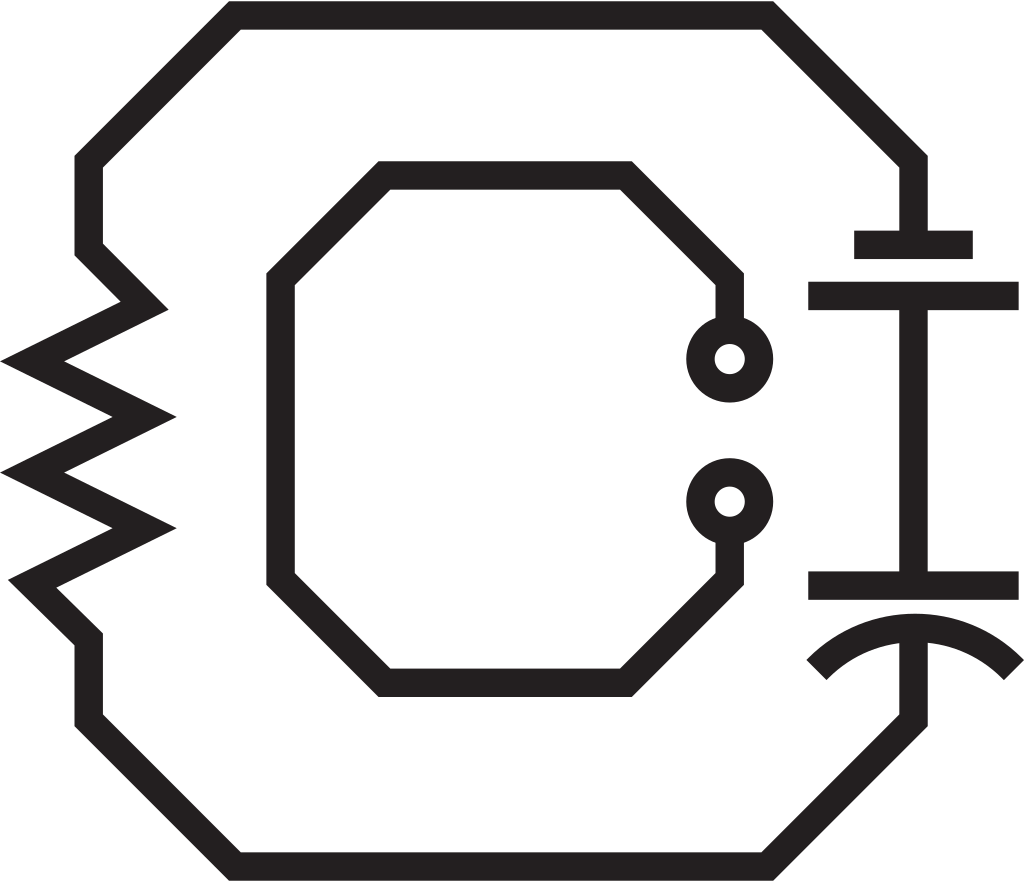
\includegraphics[height=0.635cm]{pictures/logo/c3i.png}%
    \hspace{0.25cm}%
    
\includegraphics[height=0.635cm]{pictures/logo/m1_alpha.pdf}\par
    \vspace{-0.3cm}%
    \textcolor{UDSgreenSolidarite}{%
        \noindent\rule{\textwidth}{1pt}%
    }%
}%

\defbeamertemplate*{footline}{mytheme}{%
    \leavevmode%
    \hbox{%
        \begin{beamercolorbox}%
            [wd=.33\paperwidth, ht=2.25ex, dp=1ex, center]{author in head/foot}%
            \usebeamerfont{author in head/foot}%
                \initials
        \end{beamercolorbox}%
        \begin{beamercolorbox}%
            [wd=.34\paperwidth, ht=2.25ex, dp=1ex, center]%
            {title in head/foot}%
            \usebeamerfont{title in head/foot}%
                \textbf{\inserttitle}%
        \end{beamercolorbox}%
    }%
    \begin{beamercolorbox}%
        [wd=.33\paperwidth, ht=2.25ex, dp=1ex, right]%
        {date in head/foot}%
        \hfill\usebeamerfont{date in head/foot}%
            \today{}%
        \hfill%
        \insertframenumber{} / \inserttotalframenumber%
        \hspace*{2ex}%
    \end{beamercolorbox}%
}%


%!TEX root = ../presentation.tex 


% ---------------------------------------------------------------------------
%  PACKAGES
% ---------------------------------------------------------------------------
\usepackage{tikz}        
\usepackage{etoolbox}     
\usepackage{ifthen}       
% ---------------------------------------------------------------------------
%  GLOBAL DATA
% ---------------------------------------------------------------------------
\newcount\IceSecNum        % counts the *current* section number
\IceSecNum=0               % start at zero

\newcommand{\TotalSecs}{16} % <-- Number of level/section
\newcommand{\IcebergImg}{pictures/iceberg/iceberg-background.png}

% ---------------------------------------------------------------------------
%  TEXT COLOR
% ---------------------------------------------------------------------------
\RequirePackage{xcolor}
\newcommand{\UpdateIcebergTocColor}{%
  \ifnum\IceSecNum<4
      \colorlet{IceFg}{black}% sky & ice
  \else\ifnum\IceSecNum<5
      \colorlet{IceFg}{gray!20!white}% mid‑blue water
  \else
      \colorlet{IceFg}{white}% deep ocean
  \fi\fi
  % apply to all TOC elements we’ll show
  \setbeamercolor{section in toc}{fg=IceFg}%
  \setbeamercolor{subsection in toc}{fg=IceFg}%
  \setbeamercolor{section in toc shaded}{fg=IceFg}%
  \setbeamercolor{subsection in toc shaded}{fg=IceFg}%
}

% ---------------------------------------------------------------------------
%  BACKGROUND TEMPLATE (called for every section title slide)
% ---------------------------------------------------------------------------
\newcommand{\icebergbackground}{%
  % Shift amount = –(section‑1) × (paperheight / TotalSecs)
        \pgfmathsetmacro{\t}{(\IceSecNum-1)/(\TotalSecs-1)}
        \pgfmathsetmacro{\ease}{1/(1+exp(-4*(\t-0.85)))}
        \pgfmathsetmacro{\yShift}{\ease*2872}
  %
  \usebackgroundtemplate{%
    \begin{tikzpicture}[remember picture,overlay]
      \node[anchor=north west, xshift=-10pt] at (current page.north west)
            [yshift=\yShift]  % scroll down as \IceSecNum grows
            {\includegraphics[width=\paperwidth+10pt]{\IcebergImg}};
    \end{tikzpicture}}}

% ---------------------------------------------------------------------------
%  HOOK: increment counter every time \section is called
% ---------------------------------------------------------------------------
\pretocmd{\section}{\global\advance\IceSecNum by 1\relax}{}{}

% ---------------------------------------------------------------------------
%  TOC COLUMN MACRO
% ---------------------------------------------------------------------------


\newcommand{\RightSideTOC}{%
 \UpdateIcebergTocColor
  \begin{columns}[T] % [T] aligns the tops
    \column{.85\textwidth}%
          {\raggedleft
        \tableofcontents[
        sectionstyle=shaded/show,
        subsectionstyle=show/show,
        hideothersubsections,
          sections={
            \number\numexpr\IceSecNum-1\relax,
            \number\IceSecNum,
            \number\numexpr\IceSecNum+1\relax
          }
        ]
        }
    \column{.15\textwidth}%
        %\vfill\centering\maketoctitleheader\vfill

  \end{columns}}






% --------------- BUILD SETTINGS ----------------
\pdfcompresslevel=2
\pdfobjcompresslevel=1


% \tikzexternalize

% \dump
\csname endofdump\endcsname
\endofdump
%mylatex




% ----------------------- BEGIN DOCUMENT ------------------------

\begin{document}

\titlebackground

\begin{frame}[plain]
    \maketitle
\end{frame}

\introbackground

\begin{frame}[plain, label=intro]
    \centering
    \Large

    \textcolor{white}{
        \LARGE{\textbf{\inserttitle}}\\
        \textbf{\textit{\insertsubtitle}}\\
        Par: \insertauthor\\
    }
    \vspace{24pt}
    \begin{tabular}{c l}
        \textcolor{UDSgreenFierte}{\faShield*}
            & \textcolor{white}{~Comment protéger une alimentation?}\\
            [0.3em]
        \textcolor{UDSgreenFierte}{\faSlidersH}
            & \textcolor{white}{~Quels sont les types de régulateurs?}\\
            [0.3em]
        \textcolor{UDSgreenFierte}{\faEquals}
            & \textcolor{white}{~À quoi sert le découplage?}\\
            [0.3em]
        \textcolor{UDSgreenFierte}{\faWaveSquare}
            & \textcolor{white}{~Comment filtrer une alimentation?}\\
            [0.3em]
        \textcolor{UDSgreenFierte}{\faProjectDiagram}
            & \textcolor{white}{~Comment conçevoir un arbre d'alimentation?}\\
    \end{tabular}
\end{frame}



% - TOC -
\maketoc

% ------------ SECTIONS -----------

\defaultbackground
%!TEX root = ../main.tex 

\section{Bonnes pratiques de schémas}


\section{Comment protéger une alimentation?}

\subsection{Protection antistatique}

\begin{frame}{Décharge Électrostatique (ESD)}
    \begin{columns}
        \begin{column}{0.66\textwidth}
            \begin{itemize}
                \item Norme IEC-61000-4-2
                \begin{itemize}
                    \item Types de décharges
                    \item Méthodologies de tests \& certification
                    \item 4 catégories de produits
                    \item Jusqu'à $\SI{\pm 8}{\kilo\volt}$ / $\SI{\pm 15}{\kilo\volt}$
                \end{itemize}
                \item Deux types de chocs statiques
                \begin{itemize}
                    \item \textbf{Contact Discharge} - Toucher directement chaque pin avec un ESD gun
                    \item \textbf{Air Discharge} - ESD gun proche du DUT jusqu'à décharge
                \end{itemize}
            \end{itemize}
        \end{column}

        \begin{column}{0.33\textwidth}
            \begin{figure}
                \centering
                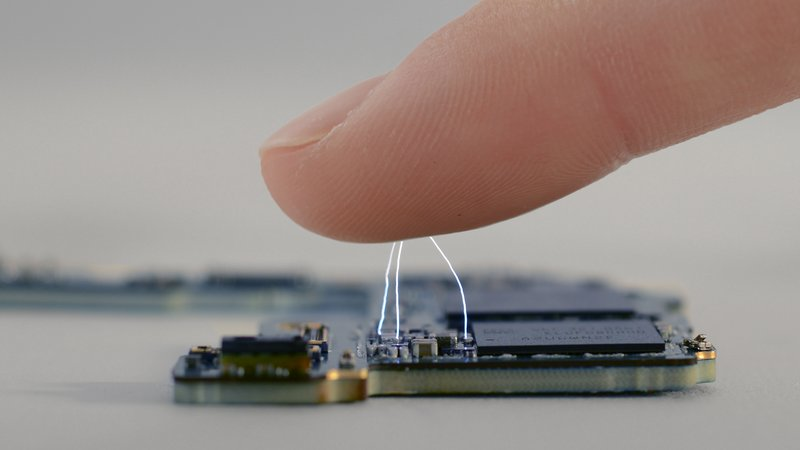
\includegraphics[width=\textwidth]{pictures/ESD-discharge-finger.png}
            \end{figure}
            \begin{figure}
                \centering
                
\includegraphics[width=0.5\textwidth]{pictures/ESD-logo.png}
            \end{figure}
        \end{column}
    \end{columns}
\end{frame}

\begin{frame}{Décharge Électrostatique - Waveform}
    \begin{columns}
        \begin{column}{0.6\textwidth}
        \end{column}
        \begin{column}{0.5\textwidth}
            \begin{itemize}
                \item Pic de courant initial
                \begin{itemize}
                    \item Rise time $\lesssim \SI{1}{\nano\second}$
                \end{itemize}
                \item $2^e$ pic
                \item Chute graduelle
            \end{itemize}
        \end{column}
    \end{columns}

    \vspace{-66pt}

    \begin{figure}
        \centering
        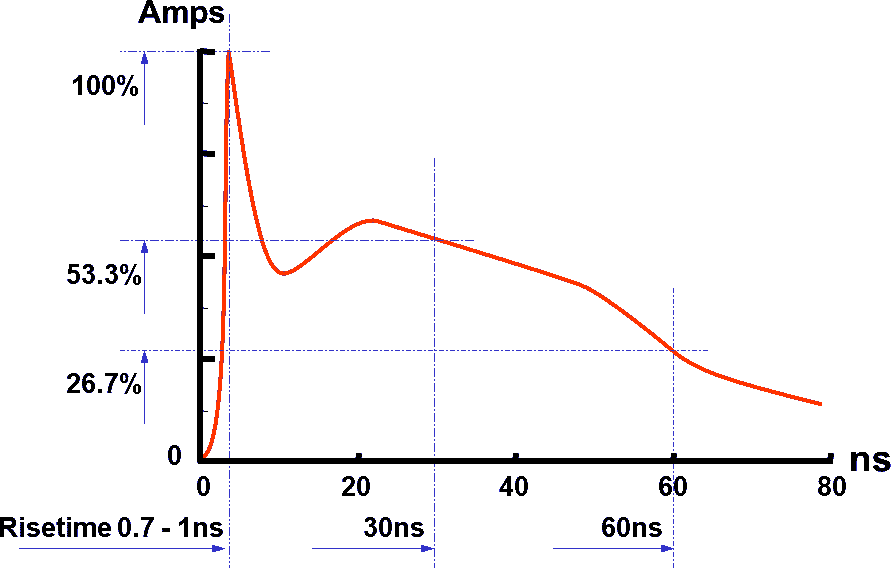
\includegraphics[width=\textwidth, height=0.8\textheight, keepaspectratio]{pictures/ESD-discharge-waveform.png}
    \end{figure}
\end{frame}

\begin{frame}{Circuit protégé antistatiquement - Zener}
    \begin{center}
    \vspace{-24pt}
    \resizebox{\textwidth}{0.8\textheight}{
    \begin{circuitikz}[american voltages]
        \draw [thick]
        (0,-3) to [short, *-] (10,-3)
        to [european resistor, l_=${LOAD}$] (10,1)
        (0,-3) to [open, v<=$V$] (0,1)
        to [short] (10,1)
        ;

        \draw [thick]
        (3, -3) to [empty ZZener diode, color=red] (3, 1);

        % Current spike as a waveform
        \draw[thick, ->] (-0.1, 2) -- (0,3) % Rising edge
        -- (0,3) -- (0.1,1.8) % First sharp drop
        -- (0.2,2.5) -- (0.3,1.9) % Second spike
        -- (0.4,2.3) -- (0.5,2.0) % Smaller oscillation
        -- (0.6,2.15) -- (0.7,2.05) % Final damping
        -- (1,2.1); % Settling

        \node[right] at (1,2.1) {$i_{\text{ESD}}(t) \rightarrow \SI{8}{\kilo\volt}$};
    \end{circuitikz}
    }
    \end{center}
\end{frame}

\begin{frame}{Diode Normale - IV Curve}
    \begin{figure}
        \centering
        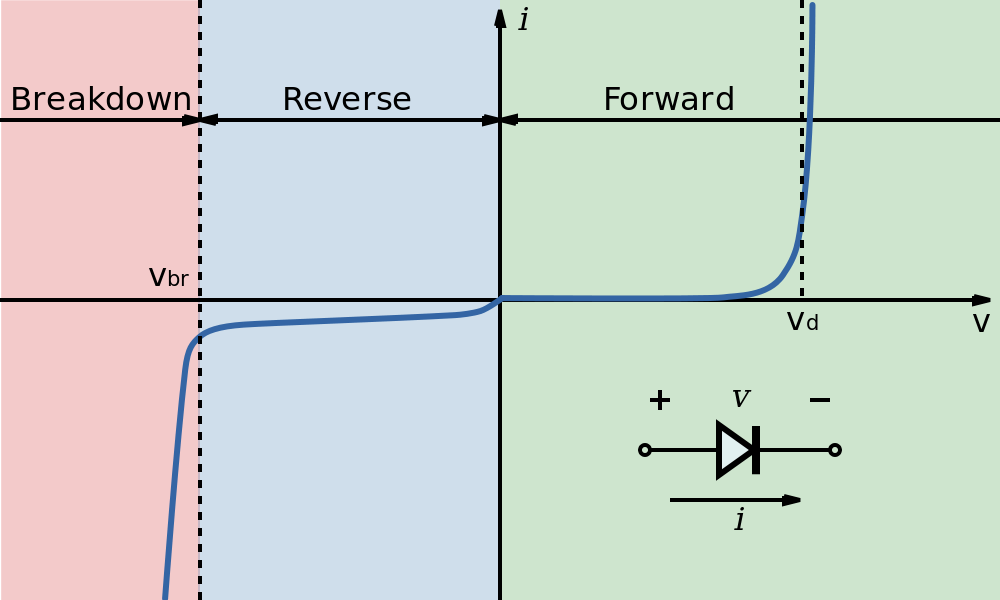
\includegraphics[width=\textwidth, height=0.8\textheight, keepaspectratio]{pictures/diode-iv-curve.png}
    \end{figure}
\end{frame}

\begin{frame}{Diode Zener}
    \begin{columns}
        \begin{column}{0.4\textwidth}
            \begin{itemize}
                \item \textbf{Faite pour être mise à l'envers!}
                \bigskip
                \item $V_Z$ contrôlé
                \item Beaucoup de courant en avalanche
                \item N'endommage pas la diode
                \bigskip
                \item Utilisé dans des références de tension
                \item Utilise comme protection antistatique
            \end{itemize}
        \end{column}
        \begin{column}{0.6\textwidth}
            \begin{figure}
                \centering
                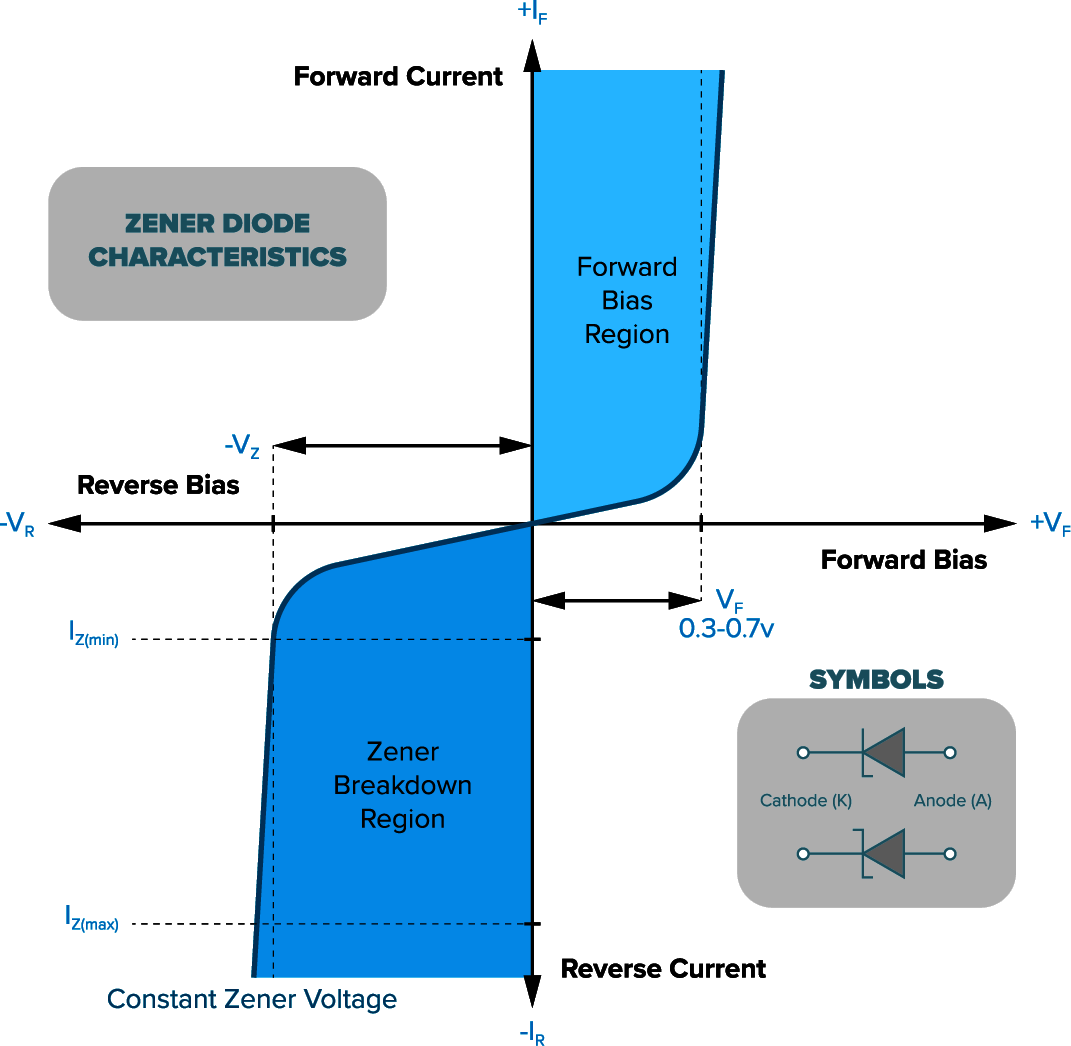
\includegraphics[width=\textwidth, height=0.8\textheight, keepaspectratio]{pictures/diode-zener-iv-curve.png}
            \end{figure}
        \end{column}
    \end{columns}
\end{frame}

\begin{frame}{Circuit protégé antistatiquement}
    \begin{center}
    \vspace{-24pt}
    \resizebox{\textwidth}{0.8\textheight}{
    \begin{circuitikz}[american voltages]
        \draw [thick]
        (0,-3) to [short, *-] (10,-3)
        to [european resistor, l_=${LOAD}$] (10,1)
        (0,-3) to [open, v<=$V$] (0,1)
        to [short] (10,1)
        ;

        \draw [thick]
        (3, -3) to [full ZZener diode, a=$\SI{15}{\volt}$] (3, 1);

        \draw[->, thick, red] 
        (1, 0.75) to[out=0, in=90] (2.75, -0.5);

        % Current spike as a waveform
        \draw[thick, ->]
           (-0.1, 2) -- (0,3)       % Rising edge
        -- (0,3) -- (0.1,1.8)       % First sharp drop
        -- (0.2,2.5) -- (0.3,1.9)   % Second spike
        -- (0.4,2.3) -- (0.5,2.0)   % Smaller oscillation
        -- (0.6,2.15) -- (0.7,2.05) % Final damping
        -- (1,2.1);                 % Settling

        \node[right] at (1,2.1) {$i_{\text{ESD}}(t) \rightarrow \SI{8}{\kilo\volt}$};
    \end{circuitikz}
    }
    \end{center}
\end{frame}


\begin{frame}{Protection avec une diode Zener}
    \begin{itemize}
        \item Clamp le pulse à $V_Z$
        \item Protège les dispositifs par apprès
        \bigskip
        \item Pas l'option la plus rapide
        \item Ne protège pas contre un pulse négatif 
    \end{itemize}

    \begin{figure}
        \centering
        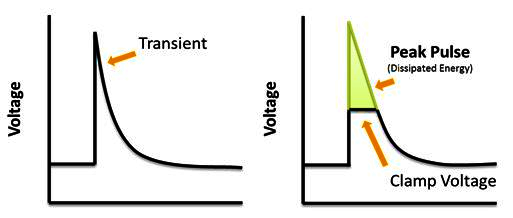
\includegraphics[width=\textwidth, height=0.5\textheight, keepaspectratio]{pictures/clamping-esd-pulse.png}
    \end{figure}
\end{frame}


\begin{frame}{Circuit protégé antistatiquement - TVS}
    \begin{center}
    \vspace{-24pt}
    \resizebox{\textwidth}{0.8\textheight}{
    \begin{circuitikz}[american voltages]
        \draw [thick]
        (0,-3) to [short, *-] (10,-3)
        to [european resistor, l_=${LOAD}$] (10,1)
        (0,-3) to [open, v<=$V$] (0,1)
        to [short] (10,1)
        ;

        \draw [thick]
        (3, -3) to [empty TVS diode, color=red] (3, 1);

        % Current spike as a waveform
        \draw[thick, ->] (-0.1, 2) -- (0,3) % Rising edge
        -- (0,3) -- (0.1,1.8) % First sharp drop
        -- (0.2,2.5) -- (0.3,1.9) % Second spike
        -- (0.4,2.3) -- (0.5,2.0) % Smaller oscillation
        -- (0.6,2.15) -- (0.7,2.05) % Final damping
        -- (1,2.1); % Settling

        \node[right] at (1,2.1) {$i_{\text{ESD}}(t) \rightarrow \pm\SI{8}{\kilo\volt}$};

        \draw[->, thick, red] 
        (1, 0.75) to[out=0, in=90] (2.75, -0.25);

        \draw[->, thick, blue] 
        (1, -2.75) to[out=0, in=-90] (2.75, -1.75);
    \end{circuitikz}
    }
    \end{center}
\end{frame}

\begin{frame}{Diode TVS (Transient Voltage Suppression)}
    \begin{columns}
        \begin{column}{0.5\textwidth}
            \begin{itemize}
                \item \textbf{Faite pour protection antistatique!}
                \item \textbf{Bidirectionnel!!}
            \end{itemize}
        \end{column}
        \begin{column}{0.5\textwidth}
            \begin{itemize}
                \item Deux diodes Zener qui se font face
                \item \textit{iv curve} symmétrique
            \end{itemize}
        \end{column}
    \end{columns}
    \begin{figure}
        \centering
        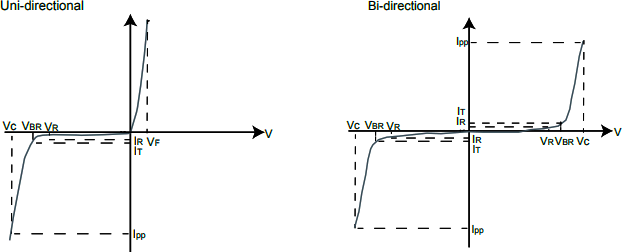
\includegraphics[width=\textwidth, height=0.55\textheight, keepaspectratio]{pictures/diode-tvs-iv-curve.png}
    \end{figure}
\end{frame}

\begin{frame}{Circuit protégé antistatiquement - Condensateur}
    \begin{center}
    \vspace{-24pt}
    \resizebox{\textwidth}{0.8\textheight}{
    \begin{circuitikz}[american voltages]
        \draw [thick]
        (0,-3) to [short, *-] (10,-3)
        to [european resistor, l_=${LOAD}$] (10,1)
        (0,-3) to [open, v<=$V$] (0,1)
        to [short] (10,1)
        ;

        \draw [thick]
        (3, -3) to [C, color=red] (3, 1);

        % Current spike as a waveform
        \draw[thick, ->] (-0.1, 2) -- (0,3) % Rising edge
        -- (0,3) -- (0.1,1.8) % First sharp drop
        -- (0.2,2.5) -- (0.3,1.9) % Second spike
        -- (0.4,2.3) -- (0.5,2.0) % Smaller oscillation
        -- (0.6,2.15) -- (0.7,2.05) % Final damping
        -- (1,2.1); % Settling

        \node[right] at (1,2.1) {$i_{\text{ESD}}(t) \rightarrow \pm\SI{8}{\kilo\volt}$};
    \end{circuitikz}
    }
    \end{center}
\end{frame}


\subsection{Protection de tension inverse}
\begin{frame}{Circuit de protection inverse - Diode}
    \begin{columns}
        \begin{column}{0.33\textwidth}
            \begin{itemize}
                \item Ne conduit que dans un sens
                \bigskip
                \item Drop de tension $V_f$
                \item $P = I \cdot V_f$
            \end{itemize}
        \end{column}
        \begin{column}{0.66\textwidth}
            \begin{center}
            \vspace{-24pt}
            \resizebox{\textwidth}{!}{
            \begin{circuitikz}[american voltages]
                \draw [thick]
                (0, 0) to [short, *-] (10, 0)
                to [european resistor, l_=${LOAD}$] (10, 5)
                (0, 0) to [open, v<=$V$] (0, 5)
                to [short] (4, 5)
                to [empty diode, color=red] (6, 5)
                to [short] (10, 5)
                ;
            \end{circuitikz}
            }
            \end{center}
        \end{column}
    \end{columns}
\end{frame}

\begin{frame}{Circuit de protection inverse - Diode Schottky}
    \begin{columns}
        \begin{column}{0.33\textwidth}
            \begin{itemize}
                \item Ne conduit que dans un sens
                \bigskip
                \item Drop de tension $V_f$ plus petite
                \item $P = I \cdot V_f$
                \bigskip
                \item Plus cher pour même rating de courant
            \end{itemize}
        \end{column}
        \begin{column}{0.66\textwidth}
            \begin{center}
            \vspace{-24pt}
            \resizebox{\textwidth}{!}{
            \begin{circuitikz}[american voltages]
                \draw [thick]
                (0, 0) to [short, *-] (10, 0)
                to [european resistor, l_=${LOAD}$] (10, 5)
                (0, 0) to [open, v<=$V$] (0, 5)
                to [short] (4, 5)
                to [empty Schottky diode, color=red] (6, 5)
                to [short] (10, 5)
                ;
            \end{circuitikz}
            }
            \end{center}
        \end{column}
    \end{columns}
\end{frame}

\begin{frame}{Circuit de protection inverse - PMOS}
    \begin{columns}
        \begin{column}{0.33\textwidth}
            \begin{itemize}
                \item Ne conduit que dans un sens
                \bigskip
                \item Drop de tension vraiment plus petite ($R_{ds_{on}} \cdot I$)
                \bigskip
                \item Tension maximale supportée
            \end{itemize}
        \end{column}
        \begin{column}{0.66\textwidth}
            \begin{center}
            \vspace{-24pt}
            \resizebox{\textwidth}{!}{
            \begin{circuitikz}[american voltages]
                \draw [thick]
                (0, 0) to [short, *-] (10, 0)
                to [european resistor, l_=${LOAD}$] (10, 5)
                (0, 0) to [open, v<=$V$] (0, 5);
                
                \draw   (4,5) node[pigfete, bodydiode, color=red, rotate=90, xscale=2, yscale=-2] (fet) {}
                (fet.G) node [anchor=south, xshift=8pt] {G}
                (fet.D) node [anchor=west, yshift=8pt] {D}
                (fet.S) node [anchor=east, yshift=8pt] {S}
                (fet.G) to [short, -*] (fet.G |- 0,0)
                (fet.D) to [short, -*] (0, 5)
                (fet.S) to (10, 5);
            \end{circuitikz}
            }
            \end{center}
        \end{column}
    \end{columns}
\end{frame}

\begin{frame}{Transistor MOSFET P-Channel (PMOS)}
    \begin{columns}
        \begin{column}{0.75\textwidth}
            \begin{center}
                $V_{gs}$ négatif!\\
                \vspace{6pt}
                $V_{gs} < -V_t$\\
                \vspace{8pt}
                Faire attention au $V_{gs_{max}}$
            \end{center}
            \vspace{24pt}

            \begin{columns}
                \begin{column}{0.5\textwidth}
                    %\textbf{Branchement normal}
                    \begin{itemize}
                        \item $V_G = \SI{0}{\volt}$
                        \item $V_{gs} = -VDD$
                        \item $-VDD < -V_t$
                        \item Conduit!
                    \end{itemize}
                \end{column}
                \begin{column}{0.5\textwidth}
                    %\textbf{Branchement inverse}
                    \begin{itemize}
                        \item $V_G = VDD$
                        \item $V_{gs} = \SI{0}{\volt}$
                        \item $\SI{0}{\volt} > -V_t$
                        \item Ne conduit pas
                    \end{itemize}
                \end{column}
            \end{columns}
        \end{column}

        \begin{column}{0.25\textwidth}
            \begin{center}
            \vspace{-24pt}
            \resizebox{!}{0.75\textheight}{
            \begin{circuitikz}[american voltages]
                
                \draw   (2,0) node[pigfete, bodydiode, xscale=1.5, yscale=1.5] (fet) {}
                (fet.G) node [anchor=east, yshift=8pt] {G}
                (fet.D) node [anchor=south, xshift=8pt, yshift=-4pt] {D}
                (fet.S) node [anchor=north, xshift=8pt, yshift=4pt] {S}
                (fet.G) to [short, -*] (fet.G |- 0, 0.4)
                (fet.D) to [short] (2, 2)
                ++(0,0) node[vcc]{VDD}
                (fet.S) to [short] (2, -1.5)
                to [R] (2, -3.5)
                to (2, -3.75) node[ground]{}
                ;

                \draw[->, thick, red] 
                (1, 0.75) to[out=90, in=180] (1.75, 1.5);

                \node[right] at (0.66, 1.66) {$V_{gs}$};
            \end{circuitikz}
            }
            \end{center}
        \end{column}
    \end{columns}
\end{frame}

\begin{frame}{Circuit de protection inverse - PMOS complèt}
    \begin{columns}
        \begin{column}{0.33\textwidth}
            \begin{itemize}
                \item Ne conduit que dans un sens
                \bigskip
                \item Drop de tension vraiment plus petite ($R_{ds_{on}} \cdot I$)
                \bigskip
                \item Supporte toutes les tensions!
            \end{itemize}
        \end{column}
        \begin{column}{0.66\textwidth}
            \begin{center}
            \vspace{-24pt}
            \resizebox{\textwidth}{!}{
            \begin{circuitikz}[american voltages]
                \draw [thick]
                (0, 0) to [short, *-] (10, 0)
                to [european resistor, l_=${LOAD}$] (10, 5)
                (0, 0) to [open, v<=$V$] (0, 5);
                
                \draw   (4,5) node[pigfete, bodydiode, rotate=90, xscale=2, yscale=-2] (fet) {}
                (fet.G) node [anchor=south, xshift=8pt] {G}
                (fet.D) node [anchor=west, yshift=8pt] {D}
                (fet.S) node [anchor=east, yshift=8pt] {S}
                (fet.G) to [R, -*] (fet.G |- 0, 0)
                (fet.D) to [short, -*] (0, 5)
                (fet.S) to (10, 5)
                (fet.G) to [short, *-] (fet.G -| 6,3)
                to [empty ZZener diode, color=red] (6, 5);
            \end{circuitikz}
            }
            \end{center}
        \end{column}
    \end{columns}
\end{frame}


\subsection{Protection de court-circuit}

\begin{frame}{Fusible}
    \begin{columns}
        \begin{column}{0.5\textwidth}
            \begin{itemize}
                \item Chauffage d'un filament central
                \item Coupe un circuit lorsque trop de courant passe
                \bigskip
                \item Usage unique
                \item Lent à agir
            \end{itemize}
            \vspace{12pt}
            \begin{figure}
                \centering
                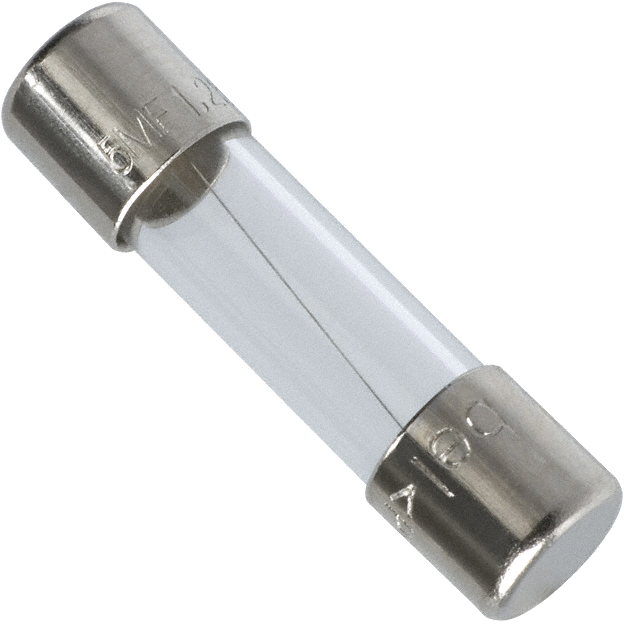
\includegraphics[width=0.33\textwidth]{pictures/fuse.png}
            \end{figure}
        \end{column}

        \begin{column}{0.6\textwidth}
            \vspace{-12pt}
            \begin{figure}
                \centering
                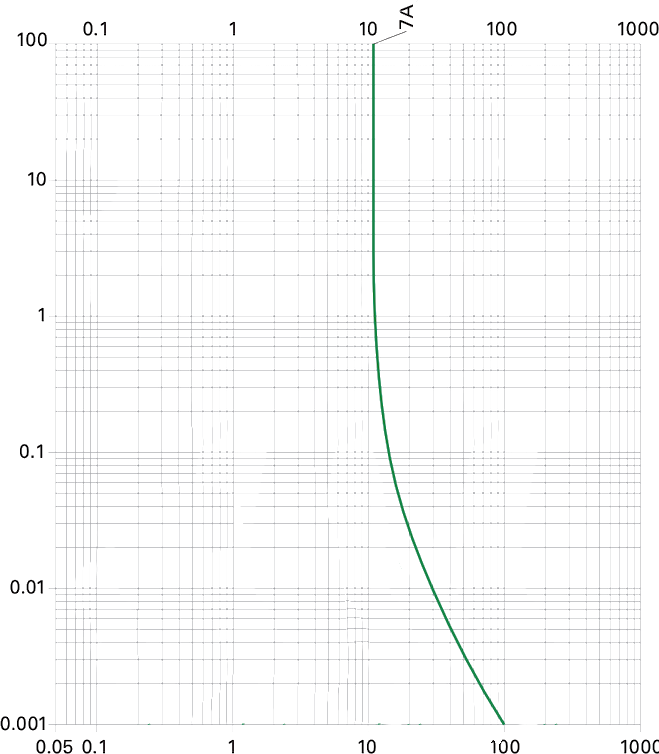
\includegraphics[width=\textwidth, height=0.75\textheight, keepaspectratio]{pictures/fuse-curve.png}
            \end{figure}
        \end{column}
    \end{columns}
\end{frame}

\begin{frame}{Polyfuse - Polyswitch - PTC - Resettable Fuse}
    \begin{columns}
        \begin{column}{0.6\textwidth}
            \begin{itemize}
                \item \textit{Positive Temperature Coefficient}
                \item Augmente sa résistance alors qu'il chauffe
                \item Utilisé comme thermistor
                \bigskip
                \item Usage multiple
                \item Lent à agir
                \item Prend du temps à se self-reset
            \end{itemize}
            \vspace{12pt}
            \begin{figure}
                \centering
                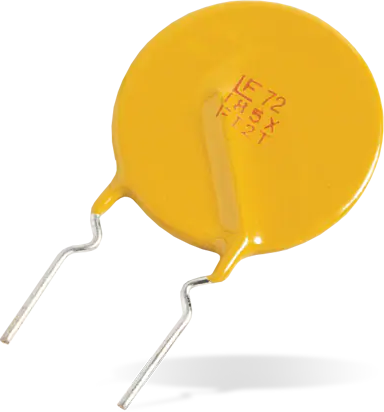
\includegraphics[width=0.25\textwidth]{pictures/polyfuse.png}
            \end{figure}
        \end{column}

        \begin{column}{0.4\textwidth}
            \begin{figure}
                \centering
                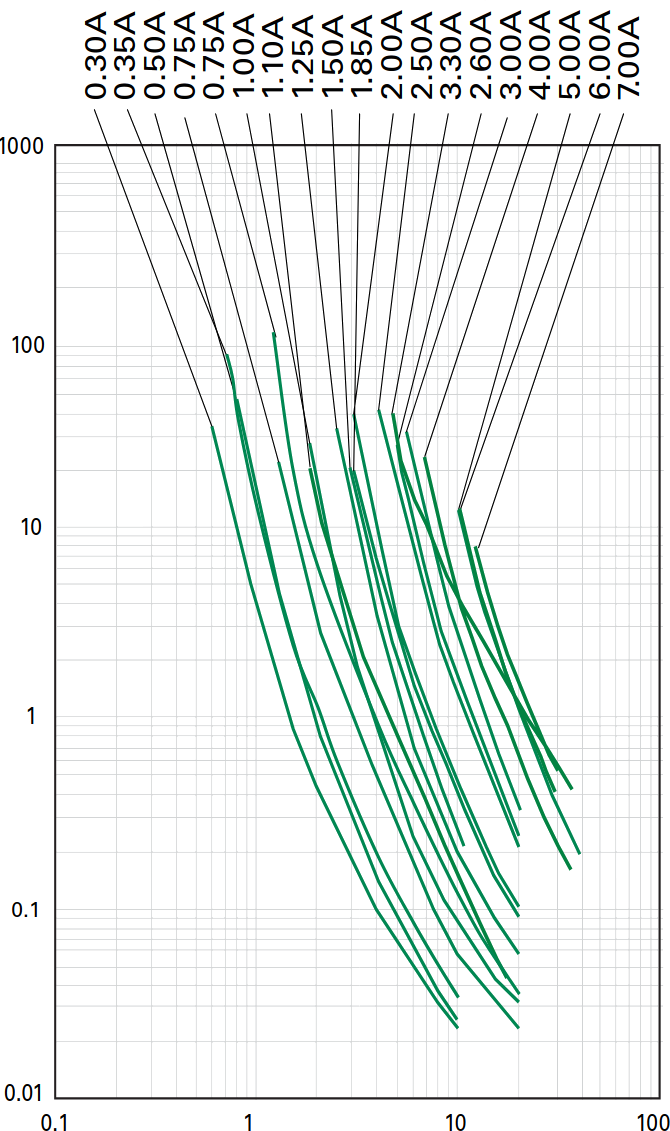
\includegraphics[width=\textwidth, height=0.75\textheight, keepaspectratio]{pictures/polyfuse-curve.png}
            \end{figure}
        \end{column}
    \end{columns}
\end{frame}

\subsection{Protection de inrush current}

\begin{frame}{Inrush Current}
    \begin{itemize}
        \item Tous les condensateurs d'un circuit sont des court-circuits
        \item Courant qui dépasse les spécifications pour charger les condensateurs
        \bigskip
        \item<2-> Spécification USB 2.0: $\SI{10}{\micro\farad}$
    \end{itemize}

    \vfill
    \begin{figure}
        \centering
        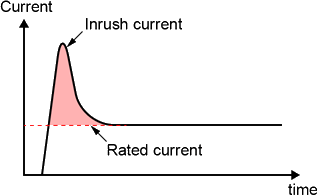
\includegraphics[height=0.55\textheight]{pictures/inrush-current.png}
    \end{figure}
\end{frame}

\begin{frame}{Inrush Current Limiter}
    \begin{columns}
        \begin{column}{0.6\textwidth}
            \textbf{Comment limiter la surge initiale?}
            \vspace{12pt}
            \begin{itemize}
                \item<1-> NTP
                \begin{itemize}
                    \item<1-> \textit{Negative Temperature Coefficient}
                    \item<1-> Conduit de plus en plus alors qu'il chauffe!
                \end{itemize}
                \bigskip
                \item<2-> Circuit de MOSFET
                \begin{itemize}
                    \item<2-> Charge d'un condensateur à la gate
                    \item<2-> Laisse passer de plus en plus de courant
                \end{itemize}
                \bigskip
                \item<3-> \textit{Soft-Start}
                \item<3-> \textit{Pre-Charge}
            \end{itemize}
        \end{column}

        \begin{column}{0.4\textwidth}
            \begin{figure}
                \centering
                \includegraphics<1->[width=0.4\textwidth]{pictures/inrush-current-limiter.png}
            \end{figure}
            \begin{figure}
                \centering
                \includegraphics<2->[width=\textwidth]{pictures/inrush-current-limiter-pmos.png}
            \end{figure}
        \end{column}
    \end{columns}
\end{frame}

\begin{frame}{Soft Start}
    \begin{columns}
        \begin{column}{0.575\textwidth}    
            \begin{itemize}
                \item Fonctionalité de certains régulateurs de tension
                \item Pente de la tension de sortie
                \item Ajustée avec un condensateur $C_{SS}$
            \end{itemize}
        \end{column}
        \begin{column}{0.4\textwidth}
            \begin{figure}
                \centering
                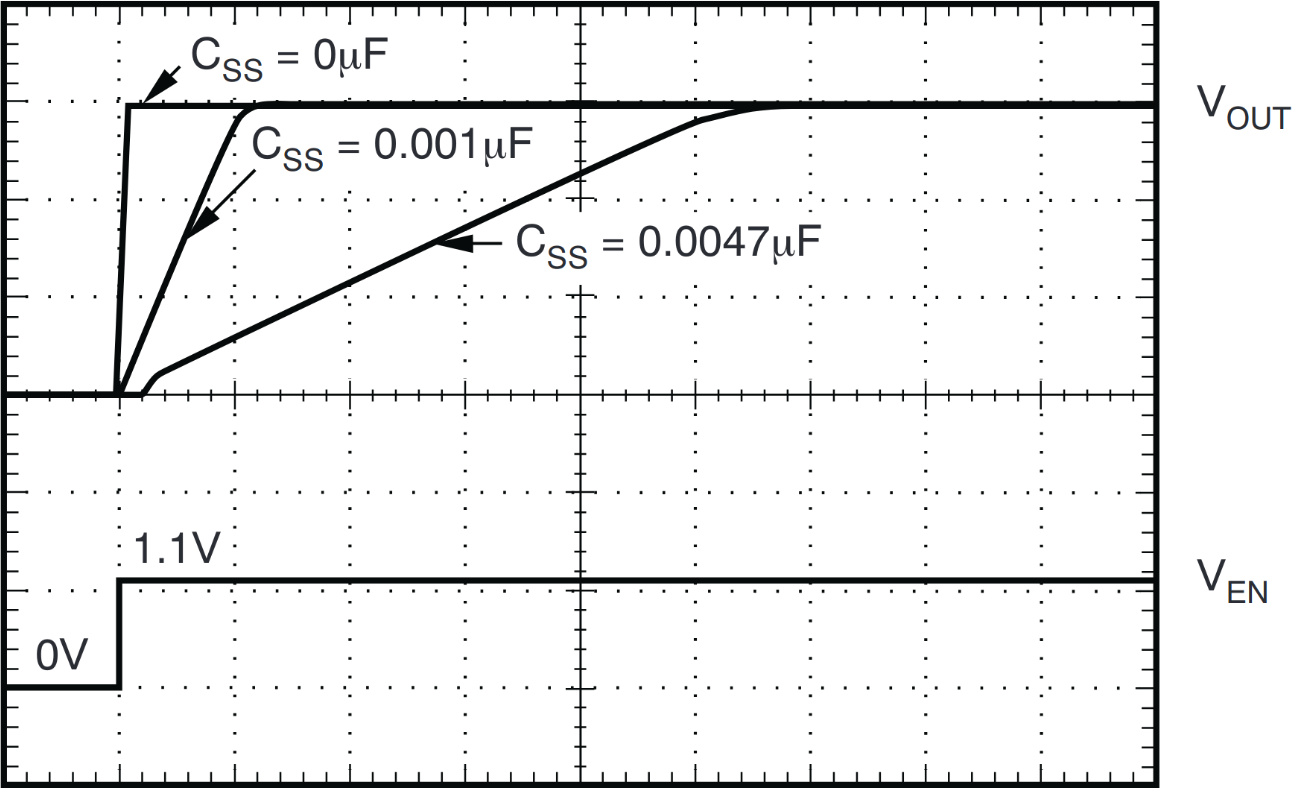
\includegraphics[width=0.9\textwidth]{pictures/ic-soft-start-curve.png}
            \end{figure}
        \end{column}
    \end{columns}
    \vfill
    \begin{figure}
        \centering
        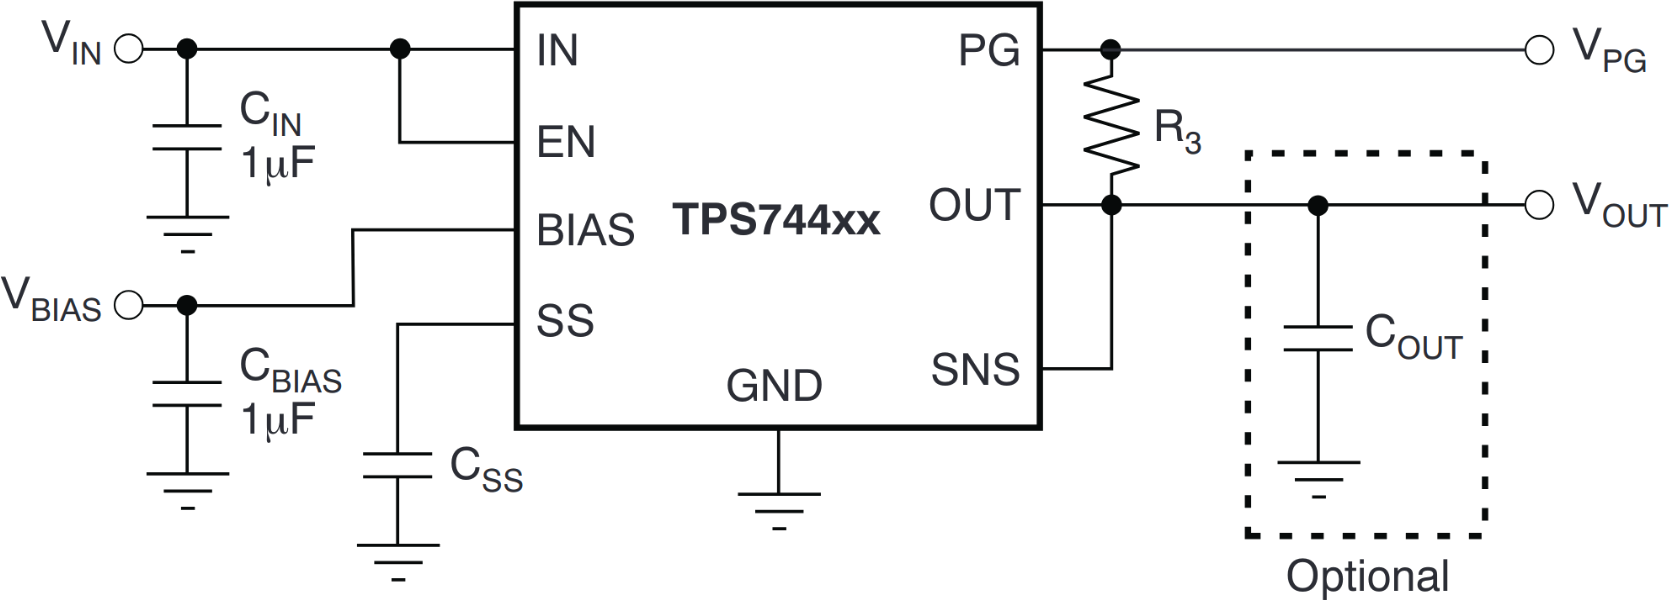
\includegraphics[width=0.66\textwidth]{pictures/ic-soft-start.png}
    \end{figure}
\end{frame}

\begin{frame}{Pre-charge}
    \begin{itemize}
        \item Pour les systèmes haut-voltage
        \item Contacteur avec une limite de courant
        \item Permet de charger les condensateurs
        \item Activation du contacteur principal après
    \end{itemize}

    \vfill

    \begin{center}
        \resizebox{!}{0.5\textheight}{
        \begin{circuitikz}[american voltages]
            \draw [thick]
            (0, 0) to [short, *-] (10, 0)
            to [european resistor, l_=${LOAD}$] (10, 5)
            (8, 5) to [short, *-] (8, 4) 
            to [C, color=red] (8, 1)
            to [short, -*] (8,0)
            (0, 0) to [open, v<=$400V$] (0, 5)
            to [short] (3, 5)
            to [normal open switch] (5, 5)
            to [short] (10, 5)
            (2, 5) to [short, *-] (2, 3)
            to [closing switch, color=red] (4, 3)
            to [R] (6, 3)
            to [short, -*] (6, 5)
            ;
        \end{circuitikz}
        }
    \end{center}    
\end{frame}

\subsection{Undervoltage Lockout}

\begin{frame}{Undervoltage Lockout (UVLO)}
\large
\centering
\begin{tabular}{c l}
    \textcolor{UDSgreenFierte}{\faPowerOff}       & Couper l'alimentation si entrée trop faible \\
    \textcolor{UDSgreenFierte}{\faBatteryQuarter} & Protection de batterie \\
    \textcolor{UDSgreenFierte}{\faPercent}        & Efficacité \\
    \textcolor{UDSgreenFierte}{\faCheckCircle}    & Garantie de fonctionnement \\
    \textcolor{UDSgreenFierte}{\faBolt}           & Du OVP (\textit{Overvoltage Protection}) ça existe aussi \\
\end{tabular}

\vfill
\begin{figure}
    \centering
    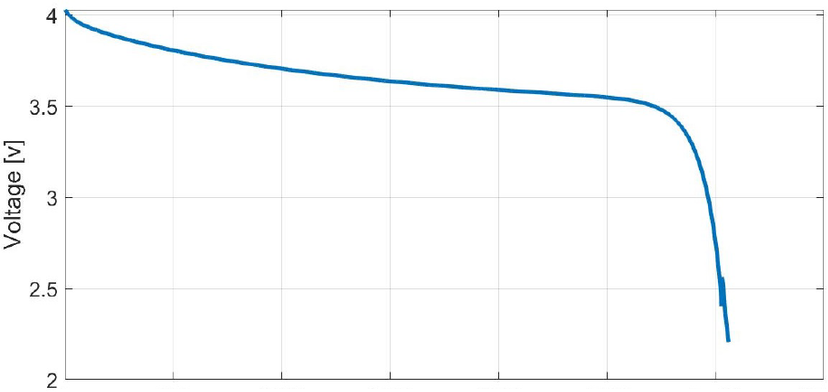
\includegraphics[width=0.66\textwidth, height=0.45\textheight, keepaspectratio]{pictures/battery-discharge-curve.png}
\end{figure}
\end{frame}

\begin{frame}{Undervoltage Lockout (UVLO) - Enable}
    \begin{columns}
        \begin{column}{0.66\textwidth}
            \begin{itemize}
                \item Batterie $V_{max} = \SI{4.2}{\volt}$
                \item Batterie $V_{min} = \SI{3.7}{\volt}$
                \item Tension EN $V_{ref} = \SI{1.2}{\volt}$
            \end{itemize}
        \end{column}

        \begin{column}{0.33\textwidth}
        \begin{center}
            Poser $R_2 = \SI{47}{\kilo\ohm}$\\
            \vspace{8pt}
            $V_{ref} = V_{min} \cdot \dfrac{R_2}{R_1 + R_2}$\\
            \vspace{6pt}
            $R_1 = $\SI{100}{\kilo\ohm}
        \end{center}
        \end{column}
    \end{columns}

    \vfill

    \begin{center}
        \resizebox{!}{0.5\textheight}{
        \begin{circuitikz}[american voltages]
        \ctikzset{multipoles/thickness=4}
        \ctikzset{multipoles/external pins thickness=2}
            % Regulator
            \draw (6, 5) node[dipchip,
                num pins=4,
                hide numbers,
                external pins width=0.3,
                external pad fraction=4 ](C){REG};
            \node [right, font=\tiny] at (C.bpin 1) {IN};
            \node [right, font=\tiny] at (C.bpin 2) {EN};
            \node [left,  font=\tiny] at (C.bpin 4) {OUT};

            % UVLO
            \draw (C.pin 2) to [short] (C.pin 2 -| 5, 5)
            to [R, l2=$R_1$ and $\SI{100}{\kilo\ohm}$, l2 halign=c] (C.pin 2 -| 2, 5) 
            to [short, -*] (C.pin 1 -| 2, 5)
            (C.pin 2 -| 5, 5) to [R, l2=$R_2$ and $\SI{47}{\kilo\ohm}$, l2 halign=c, -*] (5, 0);

            % Source & Load
            \draw
            (0, 0) to [short, *-] (10, 0)
            to [european resistor, l_=${LOAD}$] (C.pin 4 -| 10, 5)
            to [short] (C.pin 4)
            (C.pin 4 -| 9, 5) to [C, *-*] (9, 0)
            (0, 0) to [open, v<=$4.2V$] (C.pin 1 -| 0, 5)
            to [short] (C.pin 1);
        \end{circuitikz}
        }
    \end{center}  
\end{frame}


\subsection{Protection complète}

\begin{frame}{Protection complète - Circuit électrique}
    \begin{center}
        \resizebox{0.8\textwidth}{0.30\textheight}{
        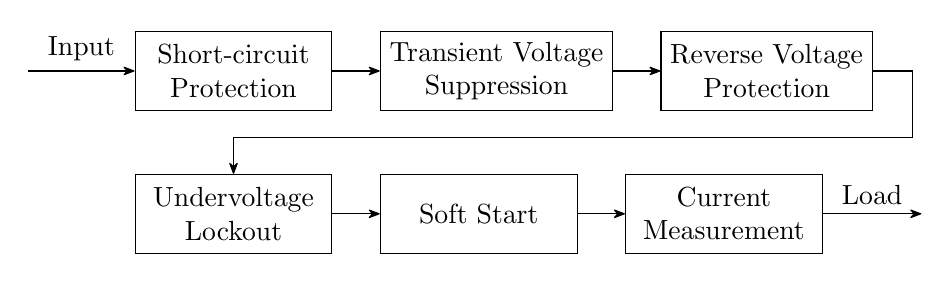
\begin{tikzpicture}[
            block/.style = {rectangle, draw, minimum height=1cm,        minimum width=2.5cm, align=center},
            node distance=0.8cm and 0.6cm,
            >={Stealth[round]}
        ]
        
        % Nodes
\node[coordinate] (inlabel) {};
\node[block, right=of inlabel] (scp) {Short-circuit\\       Protection};
\node[block, right=of scp] (tvs) {Transient Voltage\\       Suppression};
\node[block, right=of tvs] (rvp) {Reverse Voltage\\     Protection};

\node[block, below=of scp] (uvlo) {Undervoltage\\Lockout};
\node[block, right=of uvlo] (ss) {Soft Start};
\node[block, right=of ss] (cm) {Current\\Measurement};
\node[coordinate, right=of cm] (outlabel) {};

% Input arrow with label
\draw[->] ($(inlabel)+(-0.75,0.0)$) -- (scp.west) node[     midway, above] {Input};

% Top row
\draw[->] (scp) -- (tvs);
\draw[->] (tvs) -- (rvp);

% Segmented down to second row
\draw[->] 
(rvp.east)      
-- ++(0.5, 0)     
-- ++(0, -0.85)    
-| (uvlo.north);


% Bottom row
\draw[->] (uvlo) -- (ss);
\draw[->] (ss) -- (cm);

% Output arrow with label
\draw[->] (cm.east) -- ++(1.25,0) node[midway, above] {Load};
        
        \end{tikzpicture}
        }
    \end{center}
    \pause
    \vspace{-12pt}
    \begin{center}
        \resizebox{\textwidth}{!}{
        \begin{circuitikz}[american voltages]
        \ctikzset{multipoles/thickness=4}
        \ctikzset{multipoles/external pins thickness=2}
            % Regulator
            \draw (18, 5) node[dipchip,
                num pins=6,
                hide numbers,
                external pins width=0.3,
                external pad fraction=4 ](C){REG};
            \node [right, font=\tiny] at (C.bpin 1) {IN};
            \node [right, font=\tiny] at (C.bpin 2) {EN};
            \node [right, font=\tiny] at (C.bpin 3) {SS};
            \node [left,  font=\tiny] at (C.bpin 6) {OUT};

            % Soft Start
            \draw
            (C.pin 3) to [short] (C.pin 3 -| 16, 5)
            to [C, l=$C_{SS}$, -*] (16, 0);

            % UVLO
            \draw (C.pin 2) to [short, -*] (C.pin 2 -| 15, 5)
            to [R] (C.pin 2 -| 13, 5) 
            to [short, -*] (C.pin 1 -| 13, 5)
            (C.pin 2 -| 15, 5) to [R, -*] (15, 0);

            % Source & Load
            \draw
            (0, 0) to [short, *-] (24, 0)
            to [european resistor, l_=${LOAD}$] (C.pin 6 -| 24, 5)
            to [R, l=$R_{CS}$] (C.pin 6)
            (C.pin 6 -| 23, 5) to [C, *-*] (23, 0)
            (0, 0) to [open, v<=$V$] (C.pin 1 -| 0, 5);

            % TVS
            \draw
            (C.pin 1 -| 4, 5) to [C, l_=$TVS$, *-*] (4, 0)
            (6, 0) to [full TVS diode, l_=$TVS$, *-*] (C.pin 1 -| 6, 5);

            % RVP
            \draw   (C.pin 1 -| 9, 5) node[pigfete, bodydiode, rotate=90, xscale=2, yscale=-2] (fet) {}
            (fet.G) node [anchor=south, xshift=8pt] {G}
            (fet.D) node [anchor=west, yshift=8pt] {D}
            (fet.S) node [anchor=east, yshift=8pt] {S}
            (fet.G) to [R, -*] (fet.G |- 0,0)
            %(fet.D) to [short, -*] (C.pin 1 -| 0, 5)
            (fet.S) to (C.pin 1)
            (fet.G) to [short, *-] (fet.G -| 11, 3)
            to [full ZZener diode, -*] (C.pin 1 -| 11, 5);

            % Fuse Protection
            \draw
            (C.pin 1 -| 0, 5) to [wfuse, l=$FUSE$] (C.pin 1 -| 4, 5)
            %to [R, l=$R_{CS}$] (C.pin 1 -| 4, 5)
            to [short] (fet.D);
            
        \end{circuitikz}
        }
    \end{center}  
\end{frame}

\begin{frame}{Solution Miracle}
    \vspace{-12pt}
    \begin{columns}
        \begin{column}{0.33\textwidth}
            \textbf<1>{Catégorie de device:}
            \begin{itemize}
                \item<1-> \textit{eFuse}
                \item<1-> \textit{Load Switch}
                \item<1-> \textit{Ideal Diode}
            \end{itemize}
        \end{column}
        \pause
        \begin{column}{0.66\textwidth}
            \begin{center}
                \textbf{Une seule chip qui:}
            \end{center}
            \begin{columns}
                \begin{column}{0.5\textwidth}
                    \begin{itemize}
                        \item \small{RVP}
                        \item \small{TVS}
                        \item \small{Short-Circuit}
                        \item \small{Current Limit}
                        \item \small{Current Monitoring}
                    \end{itemize}
                \end{column}
                \begin{column}{0.5\textwidth}
                    \begin{itemize}
                        \item \small{Soft-Start}
                        \item \small{UVLO / OVP}
                        \item \small{Très faibles pertes}
                        \item \small{Température}
                    \end{itemize}
                \end{column}
            \end{columns}
            
        \end{column}
    \end{columns}
    \vfill
    \begin{figure}
        \centering
        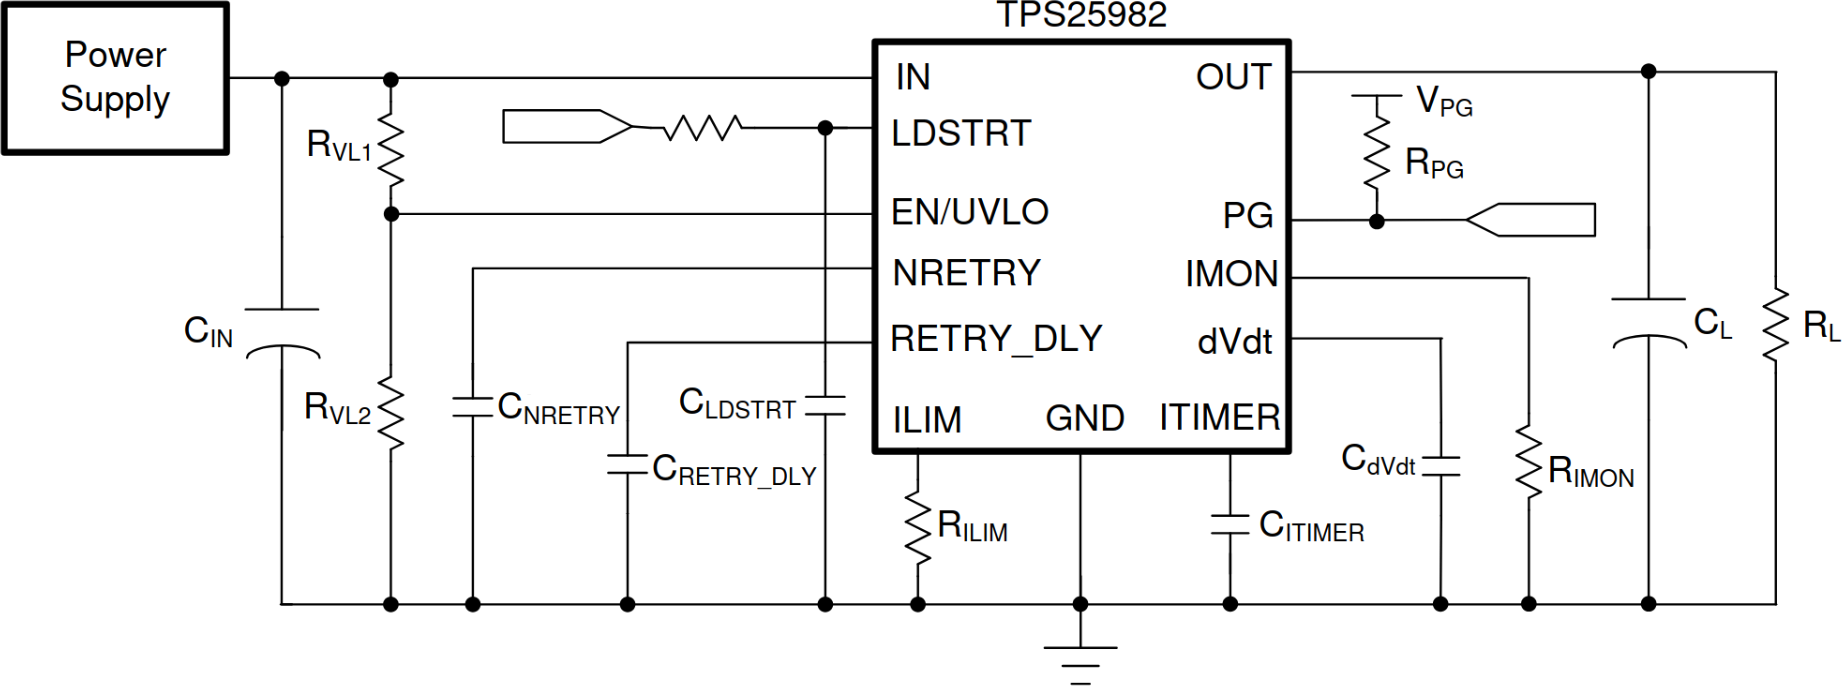
\includegraphics[width=0.75\textwidth, height=0.4\textheight, keepaspectratio]{pictures/load-switch.png}
    \end{figure}
\end{frame}


\subsection{120V}

\begin{frame}{120V}
    \begin{columns}
        \begin{column}{0.5\textwidth}
            \begin{itemize}
                \item<1-> Vivant (\textit{Live})
                \item<1-> Neutre (\textit{Neutral})
                \item<1-> Masse (\textit{Ground})
                \bigskip
                \item<2-> Pas le même GND que dans ton circuit
                \item<2-> GND du circuit provient du Neutre!
                \item<2-> \textbf{NE PAS CONNECTER ENSEMBLE}
            \end{itemize}
        \end{column}
        \begin{column}{0.5\textwidth}
            \begin{figure}
                \centering
                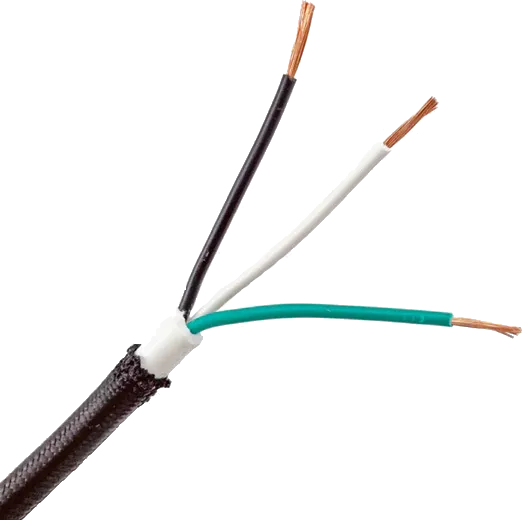
\includegraphics[width=0.75\textwidth]{pictures/120v-wire.png}
            \end{figure}
        \end{column}
    \end{columns}
\end{frame}

\begin{frame}{Connection 120V}
    \begin{center}
        \resizebox{\textwidth}{!}{
        \begin{circuitikz}[american]
            \ctikzset{voltage/american plus={\tiny $+$}};
            \ctikzset{voltage/american minus={\tiny $-$}};

            \draw (0,0) node [transformer](T){};

            \draw (T.A1) --++(-1,0);
            \draw (T.A2) --++(-1,0);
            \draw (T.B1) --++(3,0);        
            \draw (T.B2) --++(3,0);
            \draw (T.A2) to[open,v<=$\SI{25}{\kilo\volt}$](T.A1);

            \draw[thick]
            ($(T.B1)!0.5!(T.B2)-(0.7,0)$) --
            node[pos=0.25, above, inner sep=0pt](n){} ++
            (3,0);
            \draw  (n -| 2, 0) ++ (0, -0.03) -- ++ (0, -0.3) node[ground]{};

            \draw (n) to [open, v>={\footnotesize $\SI{120}{\volt}$}](T.B1);
            \draw (n) to [open, v>={\footnotesize $\SI{120}{\volt}$}](T.B2);
        \end{circuitikz}
        }
    \end{center}
\end{frame}

\begin{frame}{Grounding}
    \begin{itemize}
        \item Grounder les chassis des appareils
        \item Permet d'éviter d'avoir un chassis connecté au Live
        \item Retourne se connecter au panneau électrique
        \item Wiré séparément au Neutre
    \end{itemize}

    \vspace{-12pt}
    \begin{figure}
        \centering
        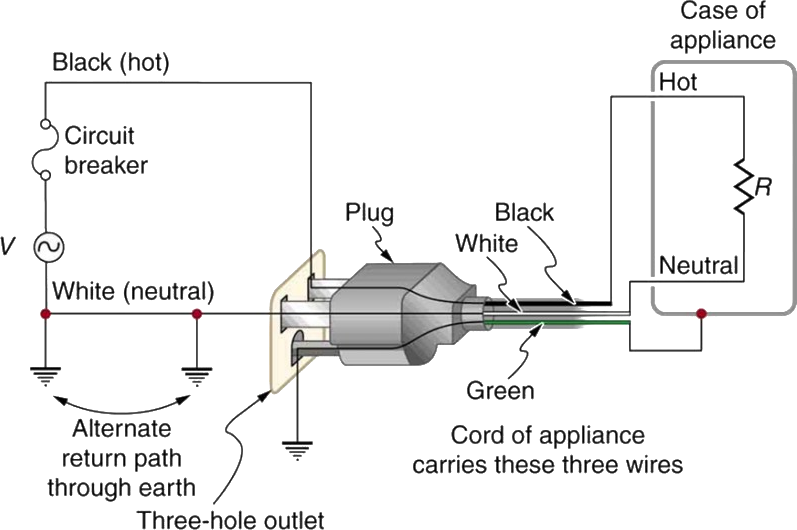
\includegraphics[width=0.66\textwidth, height=0.6\textheight, keepaspectratio]{pictures/3-wire-ac-plug.png}
    \end{figure}
\end{frame}

\begin{frame}{Grounding - Bonnes pratiques}
    \begin{columns}
        \begin{column}{0.6\textwidth}
            \begin{itemize}
                \item Garder le fil de GND plus long que les autres
                \item Mettre le LIVE plus court que les autres
                \item Toujours mettre du strain relief sur un câble
            \end{itemize}
            \vspace{-12pt}
            \begin{figure}
                \centering
                \includegraphics<1->[width=\textwidth, height=0.6\textheight, keepaspectratio]{pictures/uk-plug-wiring.png}
            \end{figure}
        \end{column}
        \begin{column}{0.4\textwidth}
            \begin{itemize}
                \item<2-> Grounder toutes les parties d'un boîtier
                \item<2-> Busbar de GND
            \end{itemize}
            \begin{figure}
                \centering
                \includegraphics<2->[width=\textwidth]{pictures/server-door-grounding.png}
            \end{figure}
        \end{column}
    \end{columns}
\end{frame}

\begin{frame}{Ground Fault Circuit Interrupter}
    \begin{columns}
        \begin{column}{0.7\textwidth}
            \begin{itemize}
                \item Mesure le courant qui passe par Live \& Neutral
                \item Coupe dès que $I_{in} \neq I_{out}$ 
            \end{itemize}
            \vspace{24pt}
            \begin{figure}
                \centering
                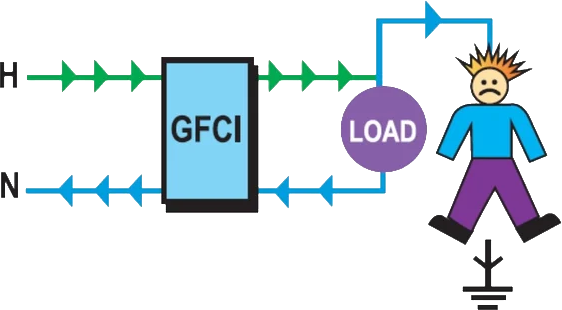
\includegraphics[width=0.75\textwidth]{pictures/gfci-example.png}
            \end{figure}
        \end{column}
        \begin{column}{0.3\textwidth}
            \begin{figure}
                \centering
                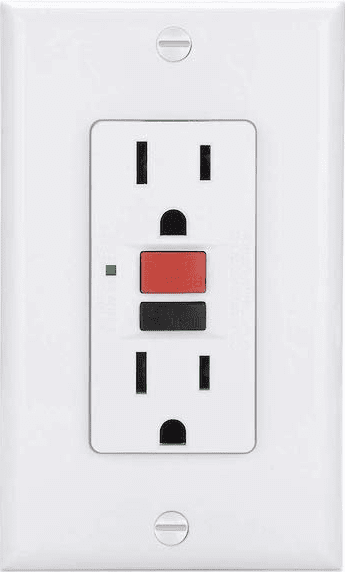
\includegraphics[width=0.6\textwidth]{pictures/gfci-outlet.png}
            \end{figure}
        \end{column}
    \end{columns}
\end{frame}
%!TEX root = ../main.tex 


\section{Quels sont les types de régulateurs?}

\begin{frame}{DC-DC - Régulateurs Linéaires vs Switching}
\renewcommand{\arraystretch}{1.4}
\begin{table}
    \centering
    \begin{tabular}{>{\color{UDSgreenSolidarite}}c c | c | c}
        \rowcolor{UDSgreenSolidarite}
        \color{white}\textbf{\faList} & \color{white}\textbf{Critère} & 
        \color{white}\textbf{Régulateur Linéaire} & 
        \color{white}\textbf{Régulateur Switching} \\
        \faDollarSign\ & \textbf{Coût}       
            & {\color{UDSgreenFierte}Faible \cmark} 
            & {\color{red}Moyen à Élevé \xmark} \\
        \faPuzzlePiece\ & \textbf{Complexité} 
            & {\color{UDSgreenFierte}Faible \cmark} 
            & {\color{red}Moyen à Élevé \xmark} \\
        \faWaveSquare\ & \textbf{Bruit}      
            & {\color{UDSgreenFierte}Faible \cmark} 
            & {\color{red}Moyen à Élevé \xmark} \\
        \faPercent\ & \textbf{Efficacité} 
            & {\color{red}Faible \xmark} 
            & {\color{UDSgreenFierte}Très Efficace \cmark} \\
        \faRandom\ & \textbf{\boldmath$V_{out}$} 
            & {\color{red}$V_{out} < V_{in}$ \xmark} 
            & {\color{UDSgreenFierte}$V_{out} \subseteq \mathbb{R}$ \cmark} \\
        \faUnlink\ & \textbf{Isolation} 
            & {\color{red} Non \xmark} 
            & {\color{UDSgreenFierte} Possible \cmark} \\
        \faThermometerHalf\ & \textbf{Température}        
            & {\color{red}Élevée \xmark}            
            & {\color{UDSgreenFierte}Faible à Moyenne \cmark} \\
        \faBolt\ & \textbf{Courant}            
            & {\color{red}Faible à Moyen \xmark}
            & {\color{UDSgreenFierte}Moyen à Élevé \cmark} \\
    \end{tabular}
\end{table}
\end{frame}


\subsection{Régulateurs Linéaires}

\begin{frame}{Régulateur Linéaire (LDO) - Résumé}
    \begin{columns}
        \begin{column}{0.5\textwidth}
            \vspace{-24pt}
            \begin{itemize}
                \item<1-> Régulateur très simple
                \begin{itemize}
                    \item<1-> IC
                    \item<1-> Pièces autours
                \end{itemize}
                \item<2-> Output très stable
                \begin{itemize}
                    \item<2-> PSRR
                \end{itemize}
                \item<3-> $V_{in} - \SI{0.3}{\volt} > V_{out}$
                \item<3-> Isolation impossible
                \item<4-> Très peu efficace
                \begin{itemize}
                    \setlength{\itemsep}{4pt}
                    \item<4-> $I_{in} = I_{out}$
                    \item<4-> $\eta = \dfrac{P_{out}}{P_{in}} = \dfrac{V_{out}}{V_{in}}$
                \end{itemize}
                \item<5-> Power dissipée en chaleur!
                \item<5-> Limite le courant
            \end{itemize}
        \end{column}

        \begin{column}{0.5\textwidth}
            \renewcommand{\arraystretch}{1.4}
            \begin{table}
            \centering
            \begin{tabular}{>{\color{UDSgreenSolidarite}}c | c}
                \rowcolor{UDSgreenSolidarite}
                \color{white}\textbf{\faList} & \color{white}\textbf{Régulateur Linéaire}\\
                \faDollarSign\ & {\color{UDSgreenFierte}Faible \cmark}\\
                \faPuzzlePiece\ & {\color{UDSgreenFierte}Faible \cmark}\\
                \ifnum\slideno>1
                \faWaveSquare\ & {\color{UDSgreenFierte}Faible \cmark}\\
                \ifnum\slideno>2 
                \faRandom\ & {\color{red}$V_{out} < V_{in}$ \xmark}\\
                \faUnlink\ & {\color{red}Non \xmark}\\
                \ifnum\slideno>3 
                \faPercent\ & {\color{red}Faible \xmark}\\
                \ifnum\slideno>4 
                \faThermometerHalf\ & {\color{red}Élevée \xmark}\\
                \faBolt\ & {\color{red}Faible à Moyen \xmark}\\
                \fi\fi\fi\fi
            \end{tabular}
            \end{table}
            \vfill
            \begin{figure}
                \centering
                \includegraphics<-2>[width=0.33\textwidth]{pictures/linear-regulator-7805.png}
            \end{figure}
        \end{column}
    \end{columns}
\end{frame}


\begin{frame}{Régulateur Linéaire - Fonctionnement}
    \vspace{-12pt}
    \begin{center}
        \resizebox{\textwidth}{0.75\textheight}{
        \begin{circuitikz}[american voltages]
            \draw [thick]
            (22, 8) to [european resistor, l=${LOAD}$] (22, 0) node [ground] {}
            (20.5, 8) to [C, *-] (20.5, 0) node [ground]{}
            (0, 8) to [C, *-] (0, 0) node [ground]{};
            \draw
            (0, 8) node [vcc, xscale=1.5, yscale=1.5] {$V_{in}$};
                
            % Feedback Voltage Divider
            \only<-2> {
                \draw [thick]
                (17, 8) to [R, *-] (17, 4) to [R] (17, 0) node[ground] {};
            }
            \only<3-> {
                \draw [thick]
                (17, 8) to [R, *-] (17, 4) to [R, v^=\LARGE{$V_{fb}$}] (17, 0) node[ground] {};
            }

            % Zener Voltage Reference
            \only<1> {
                \draw [thick]
                (5.5, 0) node[ground]{} to [empty ZZener diode] (5.5, 5) to [R, -*] (5.5, 8);
            }
            \only<2-> {
                \draw [thick]
                (5.5, 0) node[ground]{} to [empty ZZener diode, v^<={\LARGE $V_{ref}$}] (5.5, 5) to [R, f<^={\LARGE $i_Q$}, -*] (5.5, 8);
            }


            % Comparison OpAmp
            \draw [thick]
            (10, 4) node[op amp, xscale=1.5, yscale=-1.5] (amp) {}
            (amp.+) to [short, -*] (amp.+ -| 5.5, 0)
            (amp.-) to [short] (amp.- -| 7, 0)
            to [short] (7, 1) to [short] (16, 1)
            to [short] (16, 4) to [short, -*] (17, 4);

            % PMOS
            \draw [thick]
            (14, 8) node[pigfete, bodydiode, rotate=90, xscale=2, yscale=-2] (fet) {}
            (fet.G) node [anchor=south, xshift=8pt] {G}
            (fet.D) node [anchor=west, yshift=8pt] {D}
            (fet.S) node [anchor=east, yshift=8pt] {S}
            (fet.G) to [short] (fet.G |- 0, 4) to [short] (amp.out) 
            (fet.D) to [short] (0, 8)
            (fet.S) to (22, 8);

            % Soft-Start Capacitor
            \only<4-> {
                \draw [thick]
                (amp.+ -| 5.5, 0)
                to [short] (amp.+ -| 1.75, 0)
                to [C, l_={\LARGE $C_{SS}$}, color=red] (1.75, 0) node [ground] {};
            }

            % Box
            \only<-4> {
                \draw[dashed, ultra thick, rounded corners] (3, 9.5) rectangle (19, -1.5);
            }


            % Arrows
            \only<2> {
                \draw[->, thick, red] 
                (3.75, 7) to[out=-90, in=90] (3.75, 1);
            }
            \only<3> {
                \draw[->, thick, red] 
                (16.5, 4.5) to[in=0, out=180] (11, 1.5);
            }
            \only<4> {
                \draw[->, thick, red] 
                (4.75, 7.5) to[in=0, out=-90] (2.5, 5.5)
                to[in=90, out=180] (1, 3.5);
            }

        \end{circuitikz}
        }
    \end{center}  
\end{frame}

\begin{frame}{Power Supply Ripple Reduction}
    \begin{columns}
        \begin{column}{0.4\textwidth}
            \begin{center}
                $PSRR = \dfrac{\Delta V_{in}}{\Delta V_{out}}$
            \end{center}
        \end{column}
        \begin{column}{0.5\textwidth}
            \begin{center}
                $PSRR (dB) = -20 \log \left(\dfrac{\Delta V_{in}}{\Delta V_{out}}\right)$
            \end{center}
        \end{column}
    \end{columns}
    \vfill
    \begin{columns}
        \begin{column}{0.3\textwidth}
            \begin{itemize}
                \item Réduction du bruit
                \item À une fréquence
            \end{itemize}
            \pause
            \vspace{12pt}
            \begin{itemize}
                \item Graphique PSRR
                \item Dépend du courant
            \end{itemize}
        \end{column}
        \begin{column}{0.66\textwidth}
            \begin{figure}
                \centering
                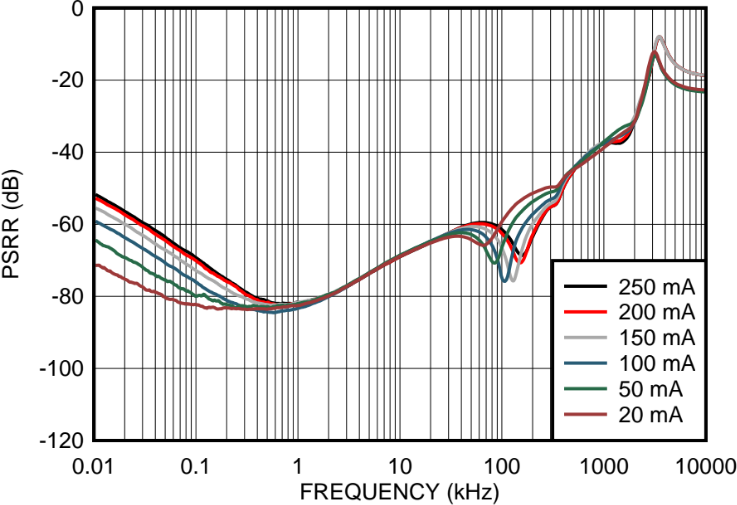
\includegraphics[width=\textwidth, height=0.6\textheight, keepaspectratio]{pictures/psrr-graph.png}
            \end{figure}
        \end{column}
    \end{columns}
\end{frame}

\begin{frame}{Quand choisir un régulateur linéaire?}
\Large
\centering
\begin{tabular}{c l}
    \textcolor{UDSgreenFierte}{\faDollarSign}   & Low-Cost \\
    [0.6em]
    \textcolor{UDSgreenFierte}{\faBolt}         & Peu de courant \\
    [0.6em]
    \textcolor{UDSgreenFierte}{\faCompress}     & Peu d'espace \\
    [0.6em]
    \textcolor{UDSgreenFierte}{\faWaveSquare}   & Bruit très important \\
    [0.6em]
    \textcolor{UDSgreenFierte}{\faPercent}      & Efficacité peu importante \\
    [1.2em]
    \textcolor{UDSgreenFierte}{\faLightbulb}    & Utiliser avec des régulateurs switching!
\end{tabular}
\end{frame}



\subsection{Régulateurs \textit{Switching}}

\begin{frame}{Régulateur Switching - Résumé}
    \begin{columns}
        \begin{column}{0.6\textwidth}
            \vspace{-12pt}
            \begin{itemize}
                \item<1-> Régulateur plus complexe
                \begin{itemize}
                    \item<1-> IC
                    \item<1-> Condensateurs \& bobines
                    \item<1-> Transistors et diodes
                \end{itemize}
                \item<1-> Plusieurs topologies
                \item<2-> Rajoute du bruit au circuit
                \begin{itemize}
                    \item<2-> Fréquence de \textit{switching}
                \end{itemize}
                \item<3-> Output très grande selon topologie
                \only<3>{
                \begin{itemize}
                        \item $V_{out} > V_{in}$
                        \item $V_{out} < \SI{0}{\volt}$
                        \item \textit{Sortie isolée possible}
                \end{itemize}
                }
                \item<4-> Extrèmement efficace
                \begin{itemize}
                    \item<4-> 80\% - 90\%
                    \only<4>{\item \textit{Courant \& Tension scale selon demande}}
                \end{itemize}
                \only<5-> {
                \item Bonne gestion thermique
                \begin{itemize}
                    \item Selon topologie
                \end{itemize}
                \item Gros courants
                }
            \end{itemize}
        \end{column}

        \begin{column}{0.4\textwidth}
            \renewcommand{\arraystretch}{1.4}
            \begin{table}
            \centering
            \begin{tabular}{>{\color{UDSgreenSolidarite}}c | c}
                \rowcolor{UDSgreenSolidarite}
                \color{white}\textbf{\faList} & \color{white}\textbf{Régulateur Linéaire}\\
                \faDollarSign\ & {\color{red}Moyen à Élevé \xmark}\\
                \faPuzzlePiece\ & {\color{red}Moyen à Élevé \xmark}\\
                \ifnum\slideno>1
                \faWaveSquare\ & {\color{red}Moyen à Élevé \xmark}\\
                \ifnum\slideno>2 
                \faRandom\ & {\color{UDSgreenFierte}$V_{out} \subseteq \mathbb{R}$ \cmark}\\
                \faUnlink & {\color{UDSgreenFierte}Possible  \cmark}\\
                \ifnum\slideno>3 
                \faPercent\ & {\color{UDSgreenFierte}Très Efficace \cmark}\\
                \ifnum\slideno>4 
                \faThermometerHalf\ & {\color{UDSgreenFierte}Faible à Moyenne \cmark}\\
                \faBolt\ & {\color{UDSgreenFierte}Moyen à Élevé \cmark}\\
                \fi\fi\fi\fi
            \end{tabular}
            \end{table}
            \vfill
            \begin{figure}
                \centering
                \includegraphics<-3>[width=0.5\textwidth]{pictures/switching-regulator-ic.png}
            \end{figure}
        \end{column}
    \end{columns}
\end{frame}

\begin{frame}{Topologies de Régulateurs Switching}
    \centering
    \Large
    \renewcommand{\arraystretch}{1.5}
    \begin{tabular}{>{\color{UDSgreenFierte}}c l | c | c}
        \rowcolor{UDSgreenSolidarite}
        & \textcolor{white}{\textbf{Topologie}} & 
        \textcolor{white}{\boldmath$V_{out}$} & 
        \textcolor{white}{\textbf{Isolation}} \\

        \faArrowDown   & \textbf{Buck}        & $V_{out} < V_{in}$                            & \xmark \\
        \faArrowUp     & \textbf{Boost}       & $V_{out} > V_{in}$                            & \xmark \\
        \faArrowsAltV  & \textbf{Buck-Boost}  & $V_{out} \subseteq \mathbb{R}$ & \xmark \\
        \faRetweet     & \textbf{SEPIC}       & $V_{out} \ge \SI{0}{\volt}$ & \xmark \\
        \faBorderStyle & \textbf{Flyback}     & $V_{out} \subseteq \mathbb{R}$ & \cmark
    \end{tabular}
\end{frame}

\begin{frame}{Régulateur Switching - Principe principal}
    \begin{itemize}
        \item Une bobine s'oppose aux changements de courant
    \end{itemize}

    \vfill
    \begin{figure}
        \centering
        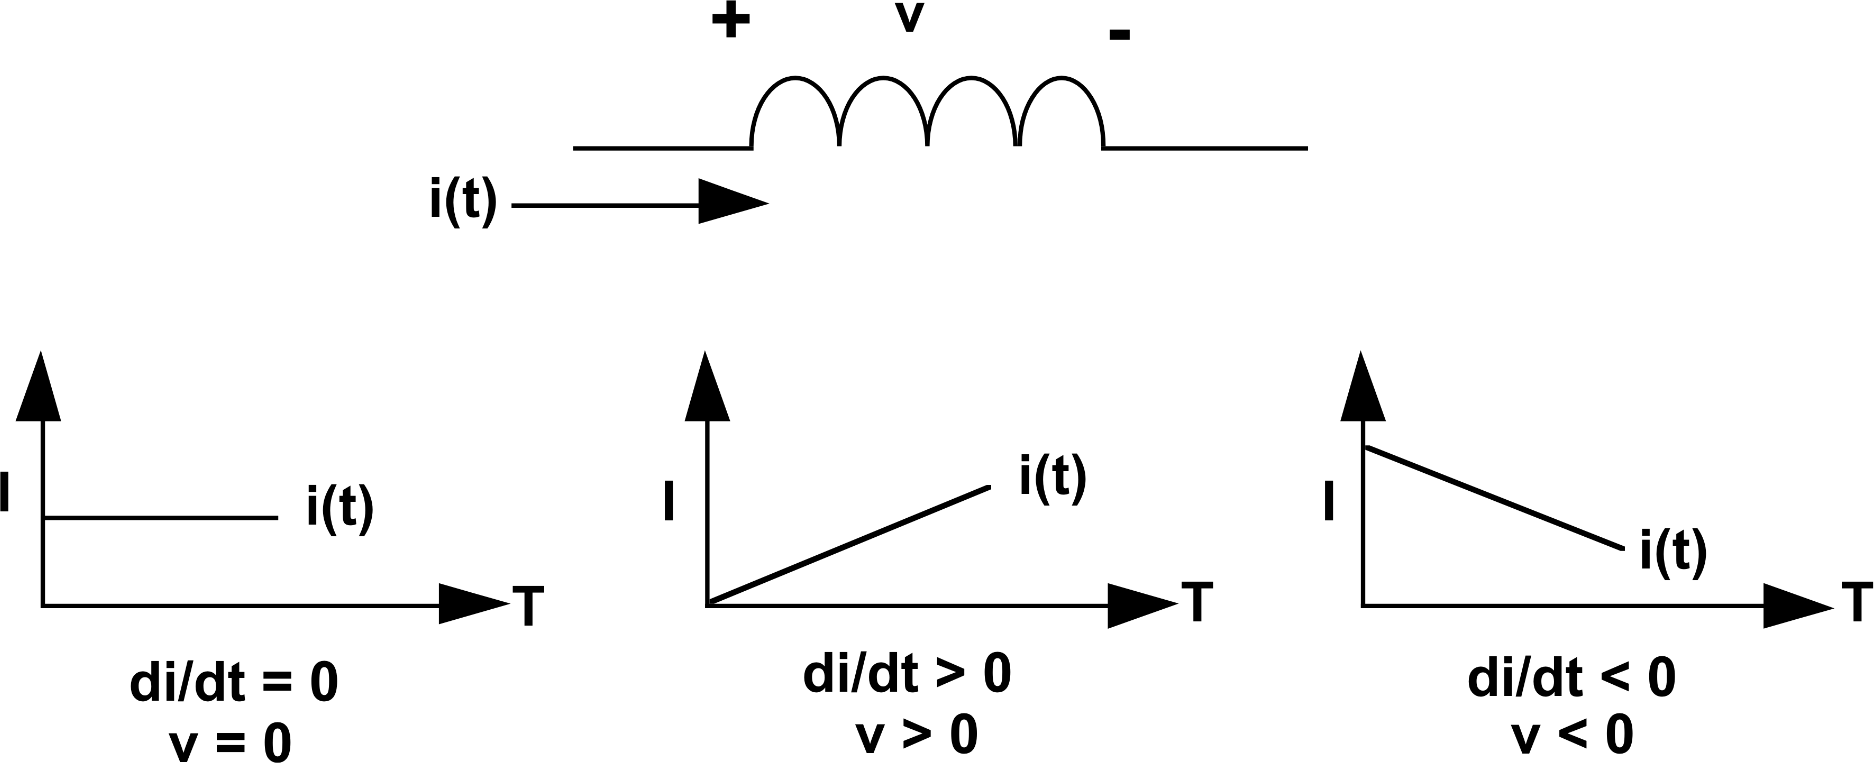
\includegraphics[width=\textwidth]{pictures/law-of-inductance.png}
    \end{figure}
\end{frame}

\begin{frame}{Régulateur Switching - Buck - Fonctionnement}
    \centering
    \resizebox{\textwidth}{!}{
    \ctikzset{inductors/scale=2}
    \begin{circuitikz}[american voltages,
        block/.style = {rectangle, draw, minimum height=1cm,        minimum width=2.5cm, align=center},
        node distance=0.8cm and 0.6cm,
        >={Stealth[round]}
    ]
        \draw [thick]
        (22, 8) to [european resistor, l=${LOAD}$] (22, 0) node [ground] {}
        (19.5, 8) to [C, *-] (19.5, 0) node [ground]{}
        (0, 8) to [C, *-] (0, 0) node [ground]{};
        \draw
        (0, 8) node [vcc, xscale=1.5, yscale=1.5] {$V_{in}$};


        % PMOS
        \only<1> {
            \draw [thick]
            (6, 8) node[pigfete, bodydiode, rotate=90, xscale=2, yscale=-2] (fet) {};
        }
        \only<2> {
            \draw [thick]
            (6, 8) node[pigfete, bodydiode, rotate=90, xscale=2, yscale=-2, color=UDSgreenFierte] (fet) {};
        }
        \only<3> {
            \draw [thick]
            (6, 8) node[pigfete, bodydiode, rotate=90, xscale=2, yscale=-2, color=red] (fet) {};
        }

        \draw [thick]
        (fet.G) node [anchor=south, xshift=8pt] {G}
        (fet.D) node [anchor=west, yshift=8pt] {D}
        (fet.S) node [anchor=east, yshift=8pt] {S}
        (fet.D) to [short] (0, 8);

        \only<1> {
            \draw[thick]
            (fet.S) to [short] (12, 8) to [american inductor] (20, 8) to [short] (22, 8);
        }
        \only<2-> {
            \draw[thick]
            (fet.S) to [short] (12, 8) to [american inductor, f>^={\Large$i$}] (20, 8) to [short] (22, 8);
        }

        % Control Block
        \draw [thick]
        (fet.G |- 0, 4) node [block, anchor=south, yshift=-8pt] (control) {\LARGE Control}
        (control.north) to [short] (fet.G);

        % Schottky Diode
        \draw [thick]
        (12, 0) node[ground]{} to [empty Schottky diode, -*] (12, 8);


        % Arrows
        \only<2> {
            \draw[->, ultra thick, red] 
            (4, 9.5) to[out=0, in=180] (8, 9.5);
            \draw[->, ultra thick, red] 
            (12.5, 9.5) to[out=0, in=180] (17, 9.5);
            \draw[->, ultra thick, red] 
            (19.5, 9.5) to[out=0, in=90] (21, 5);

            \draw[->, ultra thick, red] 
            (21, 3) to[out=-90, in=0] (19.5, -1);
            \draw[->, ultra thick, red] 
            (16, -1) to[out=180, in=0] (13, -1);
            \draw[->, ultra thick, red] 
            (9, -1) to[out=180, in=0] (5, -1);
            \draw[->, ultra thick, red] 
            (2.5, 1.5) to[out=120, in=240] (2.5, 6.5);
        }
        \only<3> {
            \draw[->, ultra thick, red] 
            (12.5, 5.5) to[out=90, in=180] (14.5, 7.5)
            to [out=0, in=180] (16.5, 7.5)
            to [out=0, in=90] (18.75, 5);
            \draw[->, ultra thick, red] 
            (18.75, 2) to[out=-90, in=0] (16.5, 0.5)
            to [out=180, in=0] (14.5, 0.5)
            to [out=180, in=-90] (12.5, 2.5);

            \draw[->, ultra thick, red] 
            (19.75, 6.5) to[out=90, in=180] (20.75, 7.5)
            to[out=0, in=90] (21.75, 6.5);
            \draw[->, ultra thick, red] 
            (21.75, 1.5) to[out=-90, in=0] (20.75, 0.5)
            to[out=180, in=-90] (19.75, 1.5);
        }
    \end{circuitikz}
    }
\end{frame}

\begin{frame}{Régulateur Switching - Buck - Waveform}
   \large
    \renewcommand{\arraystretch}{1.25}
    \begin{tabular}{>{\color{UDSgreenFierte}}c l}
        \faToggleOn   & \color{black} Le courant augmente tranquillement \\
        \color{red}\faToggleOff & \color{black} Le courant descend \\
        \faRetweet    & \color{black} Il y a toujours du courant qui s'en va vers la load \\
        \hspace{12pt}\color{red}\faBan & \hspace{12pt}\color{black} Il n'y a pas toujours du courant qui sort de la source \\
        \hspace{12pt}\faChartLine & \hspace{12pt}\color{black} $I_{out} > I_{in}$ \\
    \end{tabular}

    \vfill
    \begin{figure}
        \centering
        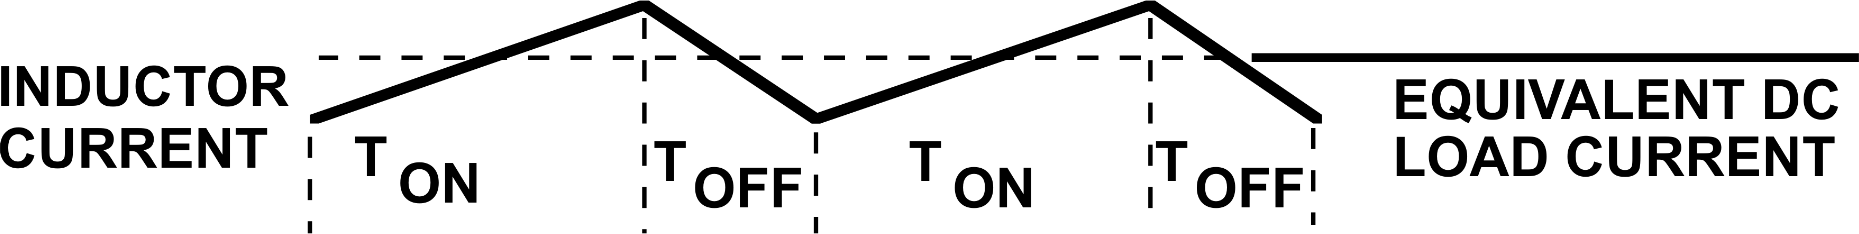
\includegraphics[width=\textwidth]{pictures/buck-switching-current.png}
    \end{figure}
\end{frame}

\begin{frame}{Régulateur Switching - Buck - Waveform}
    \vfill
    \begin{figure}
        \centering
        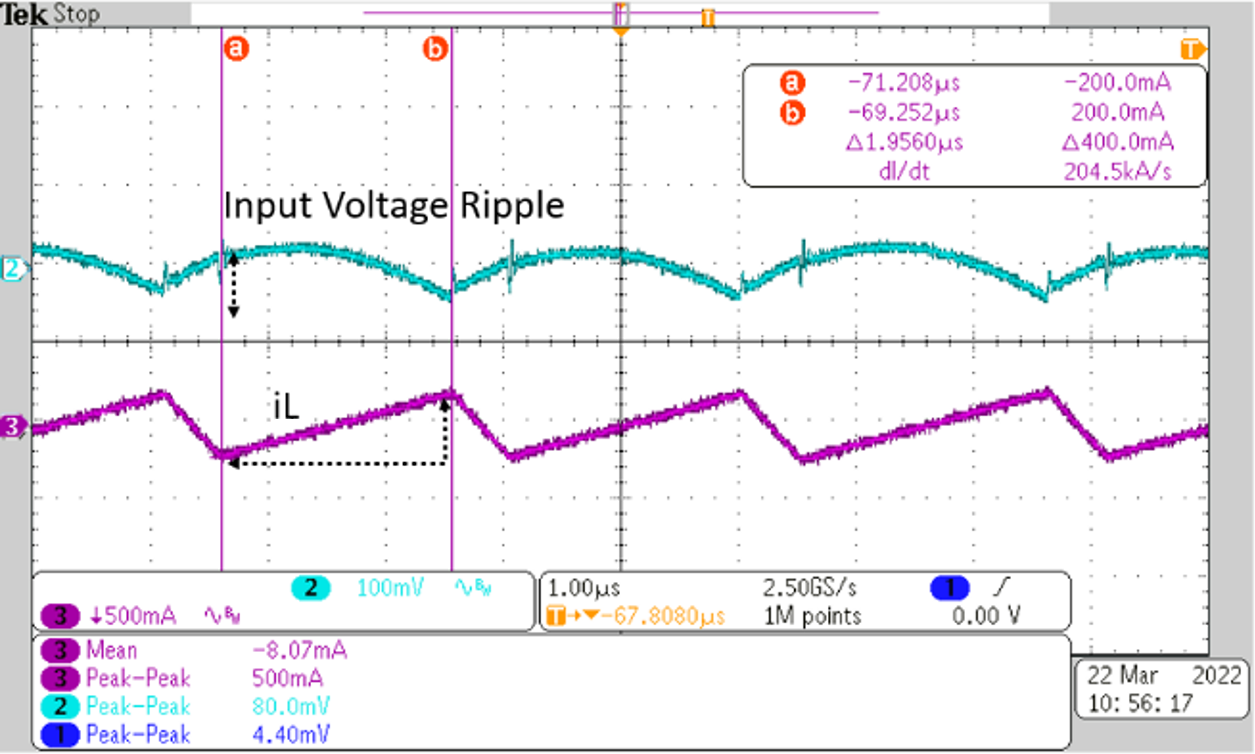
\includegraphics[width=\textwidth, height=0.8\textheight, keepaspectratio]{pictures/buck-switching-output.png}
    \end{figure}
\end{frame}


\begin{frame}{Régulateur Switching - Boost - Fonctionnement}
    \centering
    \resizebox{\textwidth}{!}{
    \ctikzset{inductors/scale=2}
    \begin{circuitikz}[american voltages,
        block/.style = {rectangle, draw, minimum height=1cm, minimum width=2.5cm, align=center},
        node distance=0.8cm and 0.8cm,
        >={Stealth[round]}
    ]
        \draw [thick]
        (22, 8) to [european resistor, l=${LOAD}$] (22, 0) node [ground] {}
        (19.5, 8) to [C, *-] (19.5, 0) node [ground]{}
        (0, 8) to [C, *-] (0, 0) node [ground]{};
        \draw
        (0, 8) node [vcc, xscale=1.5, yscale=1.5] {$V_{in}$};


        % PMOS
        \only<1> {
            \draw [thick]
            (10, 4) node[nigfete, bodydiode, xscale=2, yscale=2] (fet) {};
        }
        \only<2> {
            \draw [thick]
            (10, 4) node[nigfete, bodydiode, xscale=2, yscale=2, color=UDSgreenFierte] (fet) {};
        }
        \only<3> {
            \draw [thick]
            (10, 4) node[nigfete, bodydiode, xscale=2, yscale=2, color=red] (fet) {};
        }

        \draw [thick]
        (fet.G) node [anchor=south, xshift=8pt] {G}
        (fet.D) node [anchor=west, yshift=8pt] {D}
        (fet.S) node [anchor=east, yshift=8pt] {S}
        (fet.D) to [short, -*] (fet.D |- 0, 8)
        (fet.S) to [short] (fet.S |- 0, 0) node [ground] {};

        % Control Block
        \draw [thick]
        (fet.G -| 3.5, 4) node [block, anchor=west] (control) {\LARGE Control}
        (control.east) to [short] (fet.G);

        % Inductor
        \only<1> {
            \draw [thick]
            (0, 8) to [american inductor] (fet.D |- 0, 8);
        }
        \only<2-> {
            \draw [thick]
            (0, 8) to [american inductor, f>^={\Large$i$}] (fet.D |- 0, 8);
        }

        % Diode
        \draw [thick]
        (fet.D |- 0, 8) to [empty Schottky diode] (22, 8);


        % Arrows
        \only<2> {
            \draw[->, ultra thick, red] 
            (0.5, 5.5) to[out=90, in=180] (2.5, 7.5)
            to [out=0, in=180] (6.5, 7.5)
            to [out=0, in=90] (8.75, 5.5);
            \draw[->, ultra thick, red] 
            (8.75, 2) to[out=-90, in=0] (6.5, 0.5)
            to [out=180, in=0] (2.5, 0.5)
            to [out=180, in=-90] (0.5, 2.5);

            \draw[->, ultra thick, red] 
            (19.75, 6.5) to[out=90, in=180] (20.75, 7.5)
            to[out=0, in=90] (21.75, 6.5);
            \draw[->, ultra thick, red] 
            (21.75, 1.5) to[out=-90, in=0] (20.75, 0.5)
            to[out=180, in=-90] (19.75, 1.5);

            \draw[->, line width=4pt, UDSgreenCreativite]
            (11.5, 6) to [out=90, in=90] (11.5, 1);
        }
        \only<3> {
            \draw[->, ultra thick, red] 
            (4, 9.5) to[out=0, in=180] (8, 9.5);
            \draw[->, ultra thick, red] 
            (12.5, 9.5) to[out=0, in=180] (17, 9.5);
            \draw[->, ultra thick, red] 
            (19.5, 9.5) to[out=0, in=90] (21, 5);

            \draw[->, ultra thick, red] 
            (21, 3) to[out=-90, in=0] (19.5, -1);
            \draw[->, ultra thick, red] 
            (16, -1) to[out=180, in=0] (13, -1);
            \draw[->, ultra thick, red] 
            (9, -1) to[out=180, in=0] (5, -1);
            \draw[->, ultra thick, red] 
            (2.5, 1.5) to[out=120, in=240] (2.5, 6.5);
        }
        \only<2-> {
            \draw[->, line width=4pt, UDSgreenCreativite]
            (3, 9) to [out=0, in=180] (8, 9);
        }
    \end{circuitikz}
    }
\end{frame}


\subsection{Efficacité et Température}

\begin{frame}{Efficacité d'un régulateur linéaire}
    \begin{center}
        $\eta = \dfrac{P_{out}}{P_{in}} = \dfrac{V_{out}}{V_{in}}$

        \vfill

        \pause

        \begin{columns}
            \begin{column}{0.125\textwidth}\end{column}


            \begin{column}{0.375\textwidth}
                \centering
                \only<2-> {
                    $V_{in} = \SI{12}{\volt}$\\
                }
                \only<3-> {
                    $I_{in} = \SI{500}{\milli\ampere}$\\
                }
                \only<4-> {
                    $P_{in} = \SI{12}{\volt} \cdot \SI{500}{\milli\ampere} = \SI{6}{\watt}$\\
                }

            \end{column}

            \begin{column}{0.375\textwidth}
                \centering
                \only<2-> {
                    $V_{out} = \SI{5}{\volt}$\\
                    $I_{out} = \SI{500}{\milli\ampere}$\\
                }
                \only<4-> {
                    $P_{out} = \SI{5}{\volt} \cdot \SI{500}{\milli\ampere} = \SI{2.5}{\watt}$\\
                }
            \end{column}

            \begin{column}{0.125\textwidth}\end{column}
        \end{columns}

        \vfill
        \only<5> {
            $P_{in} - P_{out} = \SI{3.5}{\watt}$\\
            \vspace{6pt}
            $\eta = \dfrac{\SI{2.5}{\watt}}{\SI{6}{\watt}}
                  = 41.\overline{6} \% $\\
        }
        
        \only<6-> {
            $P_{in} - P_{out} = \SI{3.5}{\watt}$\\
            \vspace{6pt}
            $\eta = \dfrac{\SI{2.5}{\watt}}{\SI{6}{\watt}}      = \dfrac{\SI{5}{\volt}}{\SI{12}{\volt}}
                  = 41.\overline{6} \% $\\
        }
    \end{center}
\end{frame}

\begin{frame}{Température d'un régulateur linéaire}
    \centering
    \only<2-> {
        $\Delta T = (P_{in} - P_{out}) \cdot R_{\theta JA}$\\
        \vspace{6pt}
        $\SI{3.5}{\watt} \cdot \SI{23.9}{\celsius\per\watt} = \SI{83.85}{\celsius}$
    }

    \begin{figure}
        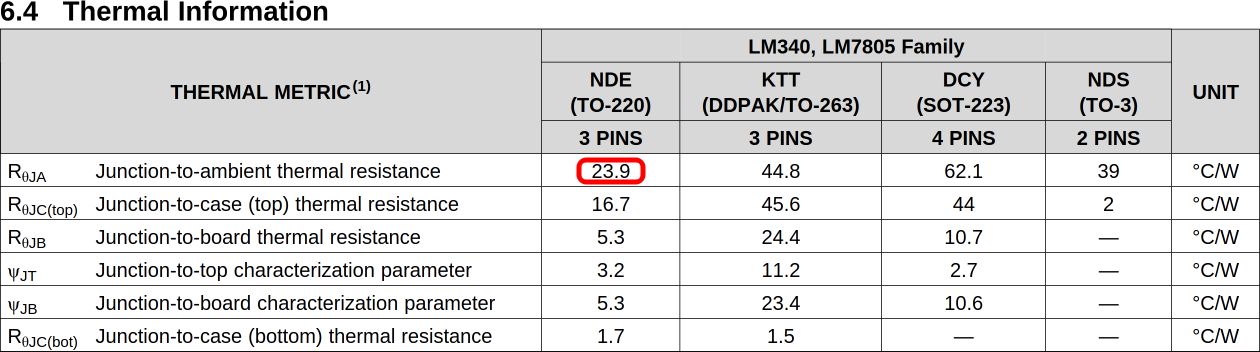
\includegraphics[width=\textwidth, height=0.75\textheight, keepaspectratio]{pictures/7805-thermal-information.png}
    \end{figure}
\end{frame}

\begin{frame}{Efficacité Régulateur Switching}
    Pour un \href{https://www.st.com/resource/en/datasheet/l6982.pdf}{ST L6982 Synchronous Monolithic Step-Down regulator}

    \begin{figure}
        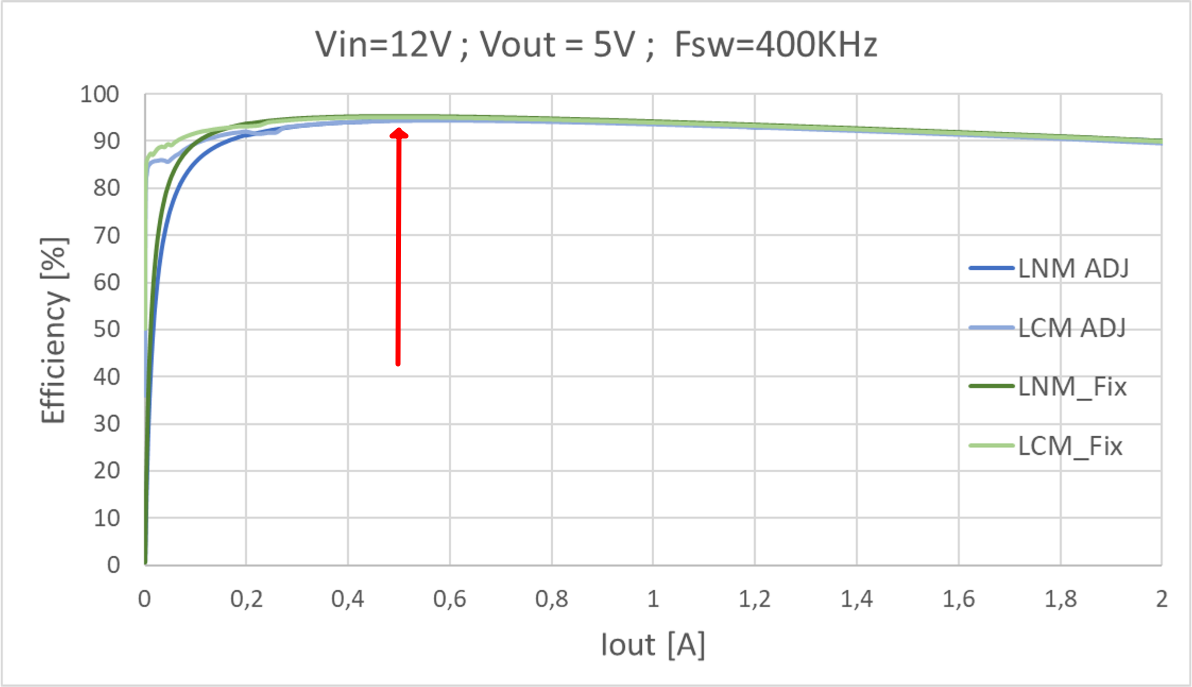
\includegraphics[width=0.66\textwidth, height=0.75\textheight, keepaspectratio]{pictures/l6982-efficiency-curve.png}
    \end{figure}
\end{frame}

\begin{frame}{Efficacité Régulateur Switching}
    \begin{columns}
        \begin{column}{0.45\textwidth}
            \centering
            \only<1-> {
                $\eta = 93\%$\\
                \vspace{12pt}
                $V_{in}  = \SI{12}{\volt}$\\
                $V_{out} = \SI{5}{\volt}$\\
                $I_{out} = \SI{500}{\milli\ampere}$\\
                $P_{out} = \SI{2.5}{\watt}$\\
            }
            \only<2-> {
                \vspace{18pt}
                $P_{in} = \dfrac{P_{out}}{\eta} = \dfrac{\SI{2.5}{\watt}}{93\%} = \SI{2.688}{\watt}$\\
                \vspace{6pt}
                $I_{in} = \frac{P_{in}}{V_{in}} = \SI{224}{\milli\ampere}$\\
            }
        \end{column}
        \begin{column}{0.55\textwidth}
            \begin{figure}
                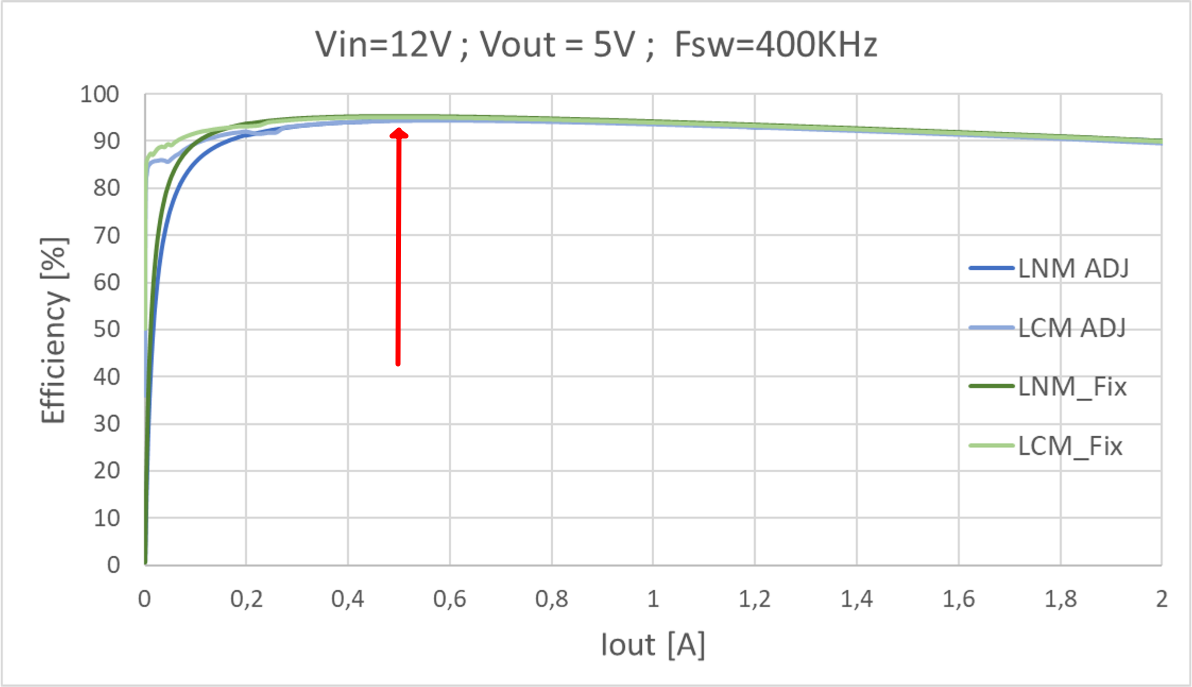
\includegraphics[width=\textwidth, height=0.75\textheight, keepaspectratio]{pictures/l6982-efficiency-curve.png}
            \end{figure}
        \end{column}
    \end{columns}
\end{frame}

\begin{frame}{Température Régulateur Switching}
    \centering
    $P_{in} - P_{out} = \SI{2.688}{\watt} - \SI{2.5}{\watt} = \SI{188}{\milli\watt}$\\
    \vspace{12pt}
    $\Delta T = (P_{in} - P_{out}) \cdot R_{\theta JA}$\\

    \vspace{24pt}
    \only<2-> {
        $\SI{0.188}{\watt} \cdot \SI{55}{\celsius\per\watt} = \SI{10.34}{\celsius}$
    }

    \vfill
    \begin{figure}
        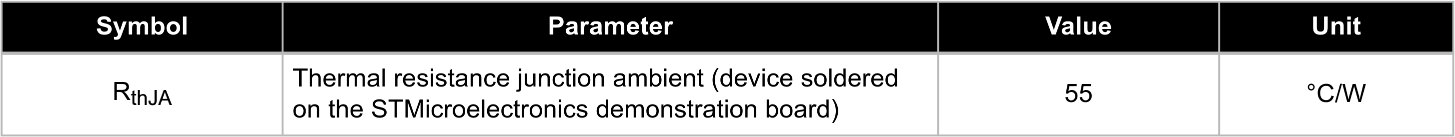
\includegraphics[width=\textwidth, height=0.75\textheight, keepaspectratio]{pictures/l6982-thermal-information.png}
    \end{figure}
\end{frame}

\begin{frame}{Sortie Régulateur Switching}
    \begin{figure}
        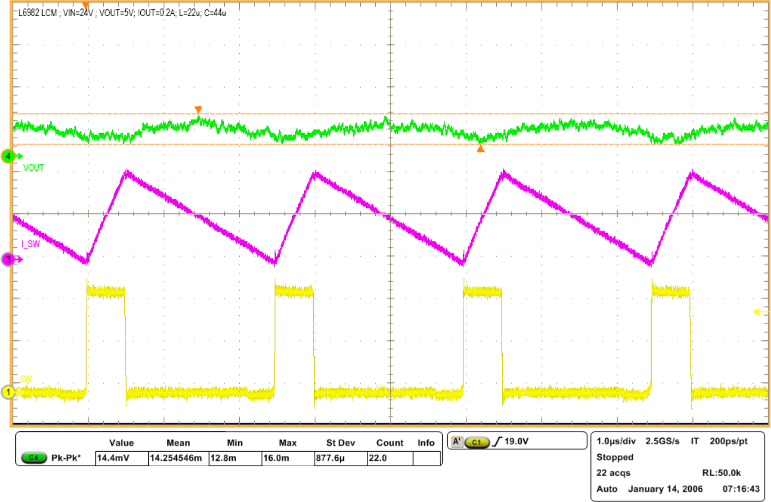
\includegraphics[width=\textwidth, height=0.75\textheight, keepaspectratio]{pictures/l6982-output.png}
    \end{figure}
\end{frame}
%!TEX root = ../main.tex 

\section{Bonnes pratiques de schéma}

\subsection{Clareté}
% Éviter tous les croisements, pas de GND dans les airs, aligner
% Utiliser la grille
% Utiliser des net names
% Quand utiliser des net locaux, globaux, power
% Inputs à gauche, output à droite
% Garder les sections modulaires, bien indiquer les sections
% Tout devrait être dans le schematics
%  - Mettre plus que pas assez
%  - Notes pour le programmeur, pour le layouteur, pour l'assembleur
%  - Tu ne devrais pas avoir à réouvrir une datasheet
% Mettre des couleurs sur les nets
% Utiliser des net classes

\subsection{Notes}
% Mettre un schéma-bloc et un arbre d'alimentation
%     Draw.io
%     Travailler en hiérarchique
% Calculer le power pour chaque bloc et page
% Mettre des notes avec tous les calculs
% Mettre des notes avec pages de datasheets
% Mettre les courbes d'efficacité etc.
% Cartouche
% Indiquer les tailles et tolérances de composantes sur le schematic
% Notes pour les pins
% - Qu'est-ce qu'elles font, comment configurer

\subsection{Testpoints et Debugging}
% Valider les boot sequences & power-sequence
% Se servir des pins flottantes
%  - Ajouter IO, LED, Testpoint, UART
% Mettre des systèmes de mesure de courant
% Met toujours plus de testpoints qu'on pense
%  - Différents types de testpoints

\subsection{Outils}
% Passer le DRC
% Les 0R sont tes amis
%  - Peut remplacer une ferrite ou une shunt
%  - Pins EN et CFG
%  - Solder Bridge Pads

\subsection{Autre}
% Bien faire son découplage
% Toujours mettre des protections
%  - ESD
%  - Power
% Export ton schematic en PDF pour l'ouvrir sans logiciel

%!TEX root = ../main.tex 

\section{Bonnes pratiques de Layout}

\subsection{Routing}
% Toujours des plans continus sous les traces
%  - Ne jamais séparer les ground planes
% Un plan de GND par plan de signal
% Faire des polygones pour le power
% Faire le stackup en fonction du fanout
% Teardrops
% Ordre de routing
% Faire attention au couplage
% Angle (30° acid trap)
% Règle du 3H

\subsection{Placement}
% Met toi plus de place que tu penses
% Placer les passives de l'autre bord
% Découplage
% Garder de l'espace sur les côtés du board
% Garder de l'espace autour des trous de vis
% Garder de l'espace avec les grosses composantes
% ESD entre l'entrée de la pin et la chip
% Orientation des chips
% Vue 3D pour le placement
% Fiducials

\subsection{Silkscreen}
% Met du texte partout
%  - Tous les testpoints, toutes les LEDs, tous les connecteurs
%  - Mettre le silkscreen plus loin
%  - Toujours avoir le silkscreen dans les mêmes orientations
% Orientation du texte

\subsection{Outils}
% Faire toutes les design rules en premier
%  - Net classes & impédance
% Grille
% Utiliser les fonctions de locking et de grouping
% Passer le DRC

\subsection{Communication avec le manufacturier}
% Fabrication Notes
% Coupon de layers
% Coupon
%  - Tous les requirements les plus difficiles à faire
%  - Si ça passe pas sur le coupon, ça passe pas sur le panel
%  - Aller voir ce que le monde mettent sur le coupon

\subsection{Autre}
% Thermal Relief
% Comment router un USB-C 2.0
% Perfectionisme (savoir quand arrêter)




% - END -

\titlebackground
\thankyouframe


% VOTE
\introbackground
\begin{frame}
    \centering
    \Large

    \textcolor{white}{\LARGE{\textbf{Vote sur le prochain PPPPP}}}\\
    \vspace{24pt}

    \only<1> {
        \textcolor{white}{
        \LARGE{\textbf{Deep-Dive sur les composantes Passives}}}\\

        \begin{itemize}
            \item \textcolor{white}{Types de condensateurs}
            \item \textcolor{white}{Derating de condensateurs}
            \item \textcolor{white}{Courbes d'impédance}
            \item \textcolor{white}{Saturation de bobines}
            \item \textcolor{white}{Normes et spécifications}
            \item \textcolor{white}{Comment choisir une composante}
        \end{itemize}
    }
    \only<2> {
        \textcolor{white}{
        \LARGE{\textbf{Bonnes pratiques de Schéma \& Layout}}}\\

        \begin{itemize}
            \item \textcolor{white}{Quoi mettre sur un silkscreen}
            \item \textcolor{white}{Notes sur un schéma}
            \item \textcolor{white}{Protections de circuit}
            \item \textcolor{white}{Comment utiliser les couches mécaniques}
            \item \textcolor{white}{Comment bien faire un BOM}
        \end{itemize}
    }
    \only<3> {
        \textcolor{white}{
        \LARGE{\textbf{Comment se déplace un signal sur un PCB}}}\\

        \begin{itemize}
            \item \textcolor{white}{Où l'impédance est la plus faible?}
            \item \textcolor{white}{Retour de courant}
            \item \textcolor{white}{Ground Bounce}
            \item \textcolor{white}{Vitesse de déplacement d'un signal}
            \item \textcolor{white}{Tout est une ligne de transmission}
        \end{itemize}
    }

    \only<4> {
        \begin{itemize}
            \item \textcolor{white}{\LARGE{\textbf{Deep-Dive sur les composantes Passives}}}
            \bigskip
            \item \textcolor{white}{\LARGE{\textbf{Bonnes pratiques de Schéma \& Layout}}}
            \bigskip
            \item \textcolor{white}{\LARGE{\textbf{Comment se déplace un signal sur un PCB}}}
        \end{itemize}
    }
\end{frame}


\end{document}
